\documentclass[
    a4paper,
    oneside,
    12pt,
    projetTutore,
    francais,
    creativecommons,
    hyperref
]{memoESPA}

\usepackage{float}
\usepackage{geometry}
\geometry{left=1.85cm,right=1.85cm,top=2.4cm,bottom=2.4cm}
\setlength{\tabcolsep}{3.5pt}
\renewcommand{\arraystretch}{1.12}

\makenomenclature
\makeindex
\newcites{refs}{WEBOGRAPHIE}
\makeatletter
\let\citerefswithmultibib\citerefs
\renewcommand{\citerefs}[1]{%
  \begingroup
  \let\@auxout\@auxoutrefs
  \citerefswithmultibib{#1}%
  \endgroup}
\makeatother
% Page de titre du rapport de projet
\title{Application web de traduction de la langue des signes en audio}
\subtitle{Reconnaissance interactive de gloses LSFB isolées par fenêtres, avec sortie textuelle contrôlée et synthèse vocale optionnelle}
\author{RATOMBOSON Tina Roédrino \\ AMBININTSOA Victor Kenitto}
\authorcopyright{RATOMBOSON Tina Roédrino et AMBININTSOA Victor Kenitto}
\datesoutenance{À compléter}
\datedepot{À compléter}
\ecole{ÉCOLE SUPÉRIEURE POLYTECHNIQUE D'ANTSIRANANA}
\mention{Sciences et Technologies de l'Information et de la Communication}
\parcours{Télécommunications et Réseaux}
\anneeU{2025--2026}
\promo{Master 1}

% Encadreurs du projet
\encadreurA{Dr.}{RANDRIAMASINORO Njakarison Menja}{Encadreur}{jury}
\encadreurB{Dr.}{RAJONIRINA Solofanja Jeannie}{Encadreur}{jury}

% Les deux encadreurs du projet sont également les seuls membres du jury.
% Aucun président ou examinateur distinct n'est déclaré.


\begin{document}
\pagenumbering{Roman}
\maketitle
\presentjury
\begin{avantpropos}

Ce rapport présente le travail réalisé dans le cadre d'un projet de Master 1 à l'École Supérieure Polytechnique d'Antsiranana. Il décrit à la fois la démarche scientifique, les choix techniques et les limites d'un prototype web consacré à la reconnaissance de gloses LSFB isolées.

Le rapport présente séparément les résultats obtenus sur le corpus et la réalisation de l'application.

\end{avantpropos}

\begin{remerciements}

Nous rendons grâce à Dieu pour la force, la santé et la persévérance qui nous ont accompagnés tout au long de ce travail.

Nous adressons nos sincères remerciements à nos parents et à nos familles pour leur soutien, leurs encouragements et leur patience.

Nous remercions également nos camarades de promotion pour leur disponibilité, leurs échanges et leur soutien.

Nous exprimons enfin notre reconnaissance à l'École Supérieure Polytechnique d'Antsiranana, aux enseignants de la mention Sciences et Technologies de l'Information et de la Communication, ainsi qu'à nos encadreurs, Monsieur RANDRIAMASINORO Njakarison Menja et Madame RAJONIRINA Solofanja Jeannie, pour les orientations apportées à la réalisation de ce projet.

\end{remerciements}

% Résumé
\begin{sommaire}{Langue des Signes Malgache, reconnaissance de signes, MediaPipe, GRU, application web}
Ce mémoire présente la reconnaissance de dix signes isolés de la Langue des Signes Malgache (LSM) et leur restitution en texte et en voix malgache. Quatre signeurs ont enregistré 400 vidéos ; les séquences d’un d’eux sont réservées au test. Chaque vidéo est convertie en points de squelette (pose et mains) extraits par MediaPipe, puis normalisée. Deux réseaux récurrents, le GRU et le LSTM, ont été entraînés et comparés à hyperparamètres identiques. Le LSTM atteint 82,0 \% d’exactitude sur le signeur de test et le GRU expérimental 92,0 \%. Le modèle final GRU, réentraîné sous la contrainte de conversion TFLite, atteint 94,0 \% ; conservant les points du corps et des mains, il a été converti au format léger TFLite (artefact de 247 Ko) et intégré à une application web : un backend FastAPI assure la reconnaissance à partir d’un court enregistrement webcam, tandis que le navigateur génère la prononciation malgache du signe reconnu. Dix essais vidéo sur l’application confirment le fonctionnement de la chaîne complète. Le prototype couvre un vocabulaire limité de signes isolés ; l’élargissement du corpus, puis la traduction de signes continus, constituent les prochaines étapes. Les résultats reposent sur un seul signeur de test et ne préjugent pas de performances générales.

\end{sommaire}

% Abstract
\begin{abstract}{Automatic recognition of isolated Malagasy Sign Language signs}{Malagasy Sign Language, sign recognition, MediaPipe, GRU, web application}
This thesis presents the recognition of ten isolated Malagasy Sign Language (LSM) signs and their restitution as text and spoken Malagasy. Four signers recorded 400 videos, and one signer is held out for testing. Each video is converted into pose and hand skeleton points extracted with MediaPipe and then normalised. Two recurrent networks, GRU and LSTM, were trained and compared under identical hyperparameters: the LSTM reaches 82.0\% accuracy on the test signer and the experimental GRU 92.0\%. The final GRU model, retrained under the TFLite conversion constraint, reaches 94.0\% accuracy; keeping both body and hand landmarks, it was converted to the lightweight TFLite format (a 247 KB artifact) and is deployed in a web application: a FastAPI backend performs the recognition from a short webcam recording, while the browser generates the Malagasy pronunciation of the recognized sign. Ten video tests on the application confirm that the complete chain works. The prototype covers a limited vocabulary of isolated signs; widening the corpus, and then translating continuous signs, are the next steps. The results rely on a single test signer and do not reflect general performance.

\end{abstract}

\tableofcontents
\addcontentsline{toc}{chapter}{\listtablename}
\listoftables
\addcontentsline{toc}{chapter}{\listfigurename}
\listoffigures
\addcontentsline{toc}{chapter}{Liste des abréviations, sigles et acronymes}
\begin{listofabbr}[4cm]
\item [ESPA] École Supérieure Polytechnique d'Antsiranana
\item [STIC] Sciences et Technologies de l'Information et de la Communication
\item [LSFB] Langue des Signes de Belgique francophone
\item [API] Application Programming Interface
\item [GRU] Gated Recurrent Unit
\item [RF] Random Forest
\item [TTS] Text-to-Speech
\item [HTTP] Hypertext Transfer Protocol
\item [WebSocket] Protocole de communication bidirectionnelle persistante
\end{listofabbr}

\addcontentsline{toc}{chapter}{Liste des symboles et unités de mesure}
\begin{listofsymbols}[4cm]
\item [$N_f$] Nombre de frames d'une séquence
\item [$T$] Température positive utilisée pour la calibration
\item [$P$] Nombre de landmarks utilisés pour une frame
\item [$C$] Nombre de classes considérées
\item [$n$] Nombre total de séquences évaluées
\item [$i$] Indice d'une séquence
\item [$c$] Indice d'une classe
\item [$m$] Indice d'un modèle ou d'une répétition de validation
\item [$j$] Indice d'une répétition ou d'un modèle de l'ensemble
\item [$y_i$] Classe réelle de la séquence $i$
\item [$\hat y_i$] Classe prédite pour la séquence $i$
\item [$p_c$] Probabilité prédite pour la classe $c$
\item [$\bar p_c$] Probabilité moyenne de la classe $c$ sur les modèles de l'ensemble
\item [$z_c$] Logit associé à la classe $c$ avant softmax
\item [$\tau_c,\tau_m,\tau_a$] Seuils de confiance, de marge et d'accord pour la politique de rejet
\item [$TP_c,FP_c,FN_c$] Vrais positifs, faux positifs et faux négatifs de la classe $c$
\item [$P_c$] Précision de la classe $c$
\item [$R_c$] Rappel de la classe $c$
\item [$F_{1,c}$] F1-score de la classe $c$
\item [$\mu$] Moyenne d'une métrique sur plusieurs graines
\item [$\sigma$] Écart-type d'une métrique
\item [$s$] Écart-type d'échantillon calculé sur plusieurs répétitions
\item [$\mathbf{1}(\cdot)$] Fonction indicatrice, égale à 1 si la condition est vraie et à 0 sinon
\item [\texttt{[32,225]}] Forme de l'entrée brute du modèle actif avant prétraitement
\item [\texttt{[32,231]}] Forme de la représentation interne fournie à la GRU
\end{listofsymbols}

\cleardoublepage
\pagenumbering{arabic}
\begin{introduction}

La Langue des Signes Malgache (LSM) est la langue utilisée par les personnes sourdes et leurs proches à Madagascar. Elle possède sa propre organisation linguistique et mobilise plusieurs parties du corps : les mains, le visage, les épaules et le regard. Dans le pays, les personnes sourdes accèdent difficilement aux services essentiels. Elles ont peu d'interlocuteurs capables de signer dans les hôpitaux, les écoles ou les administrations. Des outils de traduction adaptés au contexte local pourraient réduire considérablement cet écart.

Ce travail porte sur la LSM. Ce choix s'explique par la volonté de traiter une langue utilisée localement, encore peu représentée dans les travaux de reconnaissance automatique. Un dictionnaire de la LSM a été publié par la Fédération des Sourds de Madagascar, avec des entrées en malgache et leurs équivalents signés. Ce dictionnaire fournit une base lexicale utilisable pour construire un corpus de signes. La méthode proposée reste transposable à d'autres langues des signes dès qu'un vocabulaire équivalent est défini.

Les recherches récentes en reconnaissance de la langue des signes utilisent surtout des modèles profonds : réseaux convolutifs, Transformers, réseaux de convolution sur graphes. Ces modèles obtiennent de bons résultats sur de grands corpus. En revanche, ils demandent beaucoup de données annotées et un temps d'entraînement long. Une autre voie consiste à travailler sur les points du squelette extraits de la vidéo, plutôt que sur les images brutes. Cette représentation décrit directement la position du corps et des mains. Elle permet de comparer plusieurs modèles sur les mêmes entrées. C'est cette voie que suit le présent travail.

La question de recherche est la suivante : dans quelle mesure un modèle récurrent, entraîné sur des points du squelette extraits par MediaPipe Holistic, permet-il de traduire de façon fiable des signes isolés de la LSM ?

Le périmètre est volontairement restreint : dix signes, quatre signeurs dont un réservé au test, signes isolés, vocabulaire fermé et prototype local. Ces limites sont des choix méthodologiques. Elles garantissent la reproductibilité du pipeline et la traçabilité des décisions. La contribution visée consiste à documenter une démarche expérimentale et à fournir un prototype reproductible.

Le mémoire comporte cinq chapitres. Le premier présente l'état de l'art : spécificités de la LSM, représentations des signes, architectures de reconnaissance et travaux consacrés aux langues des signes. Le deuxième décrit la méthodologie : protocole d'enregistrement, extraction des points du squelette, préparation des données et protocole d'évaluation. Le troisième expose les expériences et les résultats de la comparaison entre LSTM et GRU, ainsi que le test de robustesse. Le quatrième présente la conception et la réalisation de l'application web, son interface et ses tests d'intégration. Le cinquième discute des limites du modèle et de l'application, puis ouvre sur les perspectives.

\end{introduction}

\chapter{État de l'art}

\section{Introduction du chapitre}

La reconnaissance automatique des langues des signes consiste à analyser des productions visuelles afin d'en identifier les unités linguistiques. Ce chapitre présente les propriétés de ces langues, les principales approches de capture et de représentation, puis les familles de modèles et des travaux représentatifs. Il se termine par une synthèse des tendances observées.

\section{La LSM comme langue multi-articulateurs}

Comme les autres langues des signes, la Langue des Signes Malgache (LSM) mobilise plusieurs articulateurs visuels et spatiaux, dont les mains, le visage, le regard et le haut du corps. Ces éléments peuvent transmettre simultanément des informations linguistiques, contrairement à la parole, qui se déploie principalement dans le temps par le canal vocal-auditif \cite{Sandler2006SignLanguageUniversals}.

Les composants manuels comprennent la configuration et l'orientation des mains, leur emplacement ainsi que leur mouvement. Lorsqu'elles sont utilisées ensemble, les deux mains peuvent jouer des rôles distincts : l'une peut notamment établir un repère spatial que l'autre réutilise. La fonction dépend du signe et du contexte ; elle n'est pas identique dans toutes les productions.

Les composants non manuels comprennent notamment les expressions du visage, le regard et les mouvements de la tête ou du tronc. Ils accompagnent la production manuelle et peuvent contribuer à l'organisation grammaticale, à la prosodie et à l'expression des intentions du signeur. La description d'une langue des signes doit donc considérer la coordination de ces composantes, plutôt que réduire le signe à une forme de la main isolée.

\section{Approches de capture et d'extraction}

La capture des signes peut s'appuyer sur des capteurs portés, tels que des gants instrumentés ou des capteurs inertiels, et sur des dispositifs optiques comme les caméras RGB ou de profondeur. Les capteurs portés mesurent des mouvements ou des configurations au moyen d'instruments attachés au corps ; les caméras observent la production sans équipement porté. Ces modalités impliquent des compromis différents en matière de matériel, de liberté de mouvement et de type d'information recueillie.

À partir d'une vidéo, les méthodes peuvent analyser directement les pixels ou en extraire des représentations intermédiaires. Les points de repère décrivent les articulations ou les parties du corps par des coordonnées, tandis que les images brutes conservent aussi l'apparence et le contexte visuel. Les représentations squelettiques sont étudiées pour la reconnaissance de langues des signes et peuvent être associées à plusieurs familles de modèles \cite{Gonfa2025Ethiopian}. MediaPipe est l'un des cadres permettant l'extraction de points de repère du corps et des mains \cite{Lugaresi2019MediaPipe,Zhang2020MediaPipeHands,Bazarevsky2020BlazePose}.

\begin{figure}[ht]
\centering
\begin{minipage}[t]{0.46\textwidth}
\centering
\includegraphics[width=\linewidth]{\detokenize{../figures/images du memoire/poselandmark-mediapipe.png}}
\par\small Points de pose du corps
\end{minipage}
\hfill
\begin{minipage}[t]{0.46\textwidth}
\centering
\includegraphics[width=\linewidth]{\detokenize{../figures/images du memoire/handlandmark-mediapipe.png}}
\par\small Points de repère d'une main
\end{minipage}
\caption{Repères corporels et manuels de MediaPipe.}
\label{fig:mediapipe-landmarks}
\end{figure}

Les coordonnées extraites peuvent ensuite être normalisées afin de limiter l'effet des différences de position, d'échelle ou de morphologie entre signeurs. Les références anatomiques et les transformations retenues varient selon les représentations et les tâches ; elles doivent être précisées et évaluées dans chaque protocole.

\section{Architectures de classification}

Plusieurs familles d'architectures peuvent classifier des séquences de points clés.

\subsection{Réseaux récurrents}

Les LSTM et les GRU sont des réseaux récurrents conçus pour représenter des séquences et leurs dépendances temporelles. Le LSTM introduit une mémoire contrôlée par des portes \cite{Hochreiter1997LSTM} ; le GRU est une autre cellule récurrente proposée dans le cadre des modèles encodeur-décodeur \cite{Cho2014GRU}. Une étude sur la langue des signes indonésienne applique MediaPipe Holistic et compare ces deux familles en temps réel ; elle rapporte 94 \% pour le LSTM et 96 \% pour le GRU \cite{Ilham2024Indonesian}. Ces résultats dépendent du corpus et du protocole propres à cette étude et ne sont pas directement généralisables.

\subsection{Transformers}

Les Transformers utilisent un mécanisme d'attention pour traiter les relations entre éléments d'une séquence \cite{Vaswani2017}. Des travaux ont étudié cette architecture pour la reconnaissance de signes arabes à partir de points de repère \cite{Alyami2023Arabic}. Cette approche constitue une alternative aux modèles récurrents pour l'analyse de séquences.

\subsection{Réseaux denses et algorithmes classiques}

Pour des données statiques ou des vecteurs agrégés, des réseaux denses (MLP) ou des algorithmes classiques comme les SVM peuvent également être étudiés. Ils constituent des points de comparaison possibles lorsque la représentation et le protocole le permettent.

\subsection{Comparaison des architectures}

Comparer plusieurs architectures sur les mêmes données et selon le même protocole permet d'isoler plus clairement l'effet des choix de modélisation. Les résultats restent toutefois dépendants de la taille et de la diversité du corpus, de la représentation choisie et des conditions d'évaluation.

\section{Comparaison de travaux sur les langues des signes}

Les études comparées ci-dessous illustrent plusieurs choix de représentation et de classification pour la reconnaissance de signes. Le tableau retient les caractéristiques utiles pour situer ces approches : langue étudiée, représentation ou modèle, et résultat ou apport méthodologique. Les performances ne sont pas directement comparables, car les corpus et les protocoles diffèrent.

\begin{table}[ht]
\centering
\small
\caption{Études sélectionnées en reconnaissance des langues des signes.}
\label{tab:comparaison-travaux-ls}
\begin{tabular}{|p{3.0cm}|p{4.3cm}|p{6.0cm}|}
\hline
Étude et langue & Approche étudiée & Résultat ou intérêt pour la comparaison \\
\hline
Ilham et al. (2024), langue des signes indonésienne \cite{Ilham2024Indonesian} & MediaPipe Holistic, comparaison LSTM--GRU en temps réel & Les auteurs rapportent 94 \% avec LSTM et 96 \% avec GRU dans leur protocole. \\
\hline
Gonfa et al. (2025), langue des signes éthiopienne \cite{Gonfa2025Ethiopian} & Représentation squelettique ; CNN-LSTM, LSTM, BiLSTM et GRU & Étudie plusieurs architectures sur une même représentation squelettique. \\
\hline
Alyami et al. (2023), langue des signes arabe \cite{Alyami2023Arabic} & Transformer et points de repère pour des signes isolés & Illustre une approche par landmarks associée à une architecture différente des réseaux récurrents. \\
\hline
Maquera et al. (2024), langue des signes péruvienne \cite{Maquera2024LSP} & Reconnaissance avec LSTM et restitution en quechua & Montre un exemple de travaux reliant reconnaissance de signes et langue parlée locale ; aucun score n'est repris ici. \\
\hline
\end{tabular}
\end{table}

Ces travaux montrent que les représentations squelettiques et plusieurs familles de modèles sont étudiées dans des contextes linguistiques distincts. Les résultats rapportés ne peuvent pas être transposés directement d'une langue ou d'un corpus à un autre ; ils servent plutôt à identifier des choix méthodologiques pertinents.

\section{Positionnement du projet}

Les travaux examinés montrent que les résultats dépendent du type de capture, de la représentation des signes, de l'architecture et du protocole expérimental. Dans ce contexte, le mémoire porte sur la comparaison de deux modèles récurrents appliqués à la Langue des Signes Malgache. Les chapitres suivants décrivent les données, le protocole et les limites nécessaires à l'interprétation de cette étude.

\section{Synthèse du chapitre}

Les approches étudiées combinent différentes modalités de capture, représentations visuelles et architectures de classification. Leurs résultats dépendent des données et des protocoles employés, ce qui rend nécessaire une description précise de ces éléments dans toute étude comparative.

\chapter{Méthodologie}

\section{Introduction du chapitre}

Ce chapitre décrit la méthode suivie pour construire et évaluer le prototype de traduction de signes isolés de la LSM. Il présente d'abord l'architecture générale du système, puis le protocole d'enregistrement du corpus. Il détaille ensuite le prétraitement des données et l'extraction des caractéristiques. Il expose enfin les architectures des modèles comparés et le protocole d'évaluation.

\section{Architecture générale du système}

Le système suit un pipeline en cinq étapes. La première est la capture vidéo d'un signe isolé produit par un signeur. La deuxième est l'extraction des points du squelette par MediaPipe Holistic, image par image. La troisième est le rééchantillonnage et la normalisation de la séquence extraite. La quatrième est la classification de la séquence par un modèle récurrent, LSTM ou GRU. La cinquième est la production du texte et de l'audio par l'application web.

\section{Constitution du jeu de données}

\subsection{Le lexique retenu}

Le prototype porte sur dix signes isolés de la LSM. Ce choix réduit la complexité du problème et permet une évaluation avec un corpus de taille modérée. Les signes couvrent plusieurs catégories : salutations, réponses simples, verbes ou états, qualificatifs et objet du quotidien.

\begin{table}[ht]
\centering
\small
\caption{Vocabulaire de signes retenu pour le prototype.}
\label{tab:lexique-lsm}
\begin{tabular}{|l|l|}
\hline
Mot en malgache & Traduction française \\
\hline
Miarahaba & Salut \\
Eny & Oui \\
Tsia & Non \\
Miezaka & Effort \\
Maheno & Entendant \\
Marenina & Sourd \\
Mora & Facile \\
Tanora & Jeune \\
Solosaina & Ordinateur \\
Maty & Mort \\
\hline
\end{tabular}
\end{table}

\subsection{Le protocole d'acquisition}

Les séquences sont enregistrées à l'aide du script \texttt{src/capture.py}. La configuration demande une résolution de 640 par 480 pixels et une cadence de 30 images par seconde ; chaque capture dure deux secondes et est précédée d'un compte à rebours de trois secondes. Ces valeurs sont des réglages demandés à la caméra et ne garantissent pas à elles seules les conditions physiques d'enregistrement. Le code ne fixe ni la distance entre le signeur et la caméra, ni l'éclairage, ni le fond.

Une vérification des fichiers du corpus confirme que les 400 vidéos sont lisibles et présentent toutes une résolution de 640 × 480 pixels, une cadence de 30 images par seconde et 60 images, soit une durée nominale de deux secondes. Chaque signeur a dix séquences pour chacun des dix signes.

Les métadonnées du corpus recensent quatre signeurs, chacun associé à dix séquences de chacun des dix signes. Le corpus comprend ainsi quarante séquences par signe et quatre cents séquences au total. Cette diversité permet d'évaluer le modèle sur un signeur qui n'a participé ni à l'entraînement ni à la validation, sans pour autant couvrir toute la variabilité des locuteurs de la LSM.

Les séances de capture se sont déroulées dans deux pièces, avec un éclairage naturel
resté constant. Le groupe comprenait trois hommes et une femme. Le signeur réservé
au test est un homme, filmé dans la seconde pièce. Ces conditions décrivent les
séances réalisées ; elles ne sont pas imposées ni contrôlées par le script de capture.

Le script affiche le signe à réaliser, lance le compte à rebours et sauvegarde la séquence. Il standardise ces étapes, mais ne vérifie pas à lui seul la qualité de chaque capture ni les conditions physiques de prise de vue.

\section{Prétraitement et extraction des caractéristiques}

\subsection{Application de MediaPipe Holistic}

MediaPipe Holistic regroupe des détecteurs de pose, des mains et du visage. Pour chaque image, il transforme l'image RGB en un ensemble de points décrits par leurs coordonnées. Le modèle de pose fournit 33 points pour le corps et le modèle des mains 21 points par main ; la documentation distingue également les repères du visage \citerefs{MediaPipeHolistic}.

Le projet utilise uniquement les points du corps et des mains, soit 33 + 21 × 2 = 75 points. Les points du visage sont écartés dans un premier temps, car ils augmentent fortement la dimension du vecteur sans que leur apport soit établi pour un vocabulaire de dix signes. Cette décision réduit la dimension de l'entrée et le coût d'entraînement. Elle pourra être révisée si les résultats montrent que certains signes se distinguent principalement par l'expression faciale.

Le visage MediaPipe comporte 468 points, soit 1\,404 coordonnées supplémentaires. Leur inclusion ferait passer le vecteur de 225 à 1\,629 valeurs par image, soit une dimension 7,24 fois plus grande. Ce calcul justifie le périmètre initial de représentation, mais ne mesure pas l'effet des points faciaux sur les performances : aucune expérience comparative avec et sans visage n'a été menée.

\subsection{Structure du vecteur d'entrée}

Chaque point est décrit par ses trois coordonnées, ce qui donne un vecteur de 75 × 3 = 225 valeurs par image. Les coordonnées sont concaténées dans l'ordre suivant : les 33 points du corps, les 21 points de la main gauche, puis les 21 points de la main droite. Cet ordre est conservé pour toutes les images et toutes les séquences ; chaque position du vecteur correspond ainsi au même point.

\subsection{Rééchantillonnage temporel}

Les séquences sont ramenées à trente images par sélection des images les plus proches des positions régulièrement espacées sur la durée de la séquence. Cette opération conserve une représentation temporelle de l'ensemble du geste et fournit une longueur fixe aux modèles.

Les fichiers d'origine contenant 60 images, ce rééchantillonnage réduit de moitié le nombre d'images fournies au modèle. Il fixe la dimension temporelle de l'entrée ; aucune comparaison directe entre 30 et 60 images n'a été réalisée pour mesurer l'information perdue ou conservée.

\subsection{Normalisation}

Les signeurs n'ont pas tous la même taille ni la même position par rapport à la caméra. Pour atténuer ces différences, les coordonnées sont centrées sur le point situé entre les deux épaules, puis divisées par la distance entre celles-ci. Cette étape est appliquée à chaque séquence ; son effet propre sur les performances n'a pas été évalué séparément.

Une vérification du tenseur prétraité confirme que, sur les 12\,000 images des 400 séquences, le centre des deux épaules est à l'origine et leur distance vaut un, à l'arrondi près des nombres flottants. Ce contrôle valide l'application de la transformation, mais ne démontre pas à lui seul une amélioration de la reconnaissance.

\subsection{Gestion des données manquantes}

Les 400 vidéos, de 60 images chacune, ont été analysées image par image avant le rééchantillonnage, avec MediaPipe Holistic 0.10.14 en mode dynamique. Le tableau indique, pour chaque signe, le nombre et la proportion d'images sans détection du groupe de points correspondant. Le dénominateur est de 2\,400 images par signe et de 24\,000 pour le total.

\begin{table}[ht]
\centering
\small
\caption{Images sans détection des landmarks par signe.}
\label{tab:non-detection-landmarks}
\begin{tabular}{|l|r|r|r|}
\hline
Signe & Pose, $n$ (\%) & Main gauche, $n$ (\%) & Main droite, $n$ (\%) \\
\hline
Miarahaba & 0 (0,00 \%) & 1\,212 (50,50 \%) & 302 (12,58 \%) \\
Eny & 0 (0,00 \%) & 1\,203 (50,12 \%) & 78 (3,25 \%) \\
Tsia & 0 (0,00 \%) & 1\,446 (60,25 \%) & 3 (0,12 \%) \\
Miezaka & 0 (0,00 \%) & 718 (29,92 \%) & 283 (11,79 \%) \\
Maheno & 0 (0,00 \%) & 1\,170 (48,75 \%) & 16 (0,67 \%) \\
Marenina & 0 (0,00 \%) & 1\,273 (53,04 \%) & 38 (1,58 \%) \\
Mora & 0 (0,00 \%) & 1\,216 (50,67 \%) & 136 (5,67 \%) \\
Tanora & 0 (0,00 \%) & 1\,180 (49,17 \%) & 398 (16,58 \%) \\
Solosaina & 0 (0,00 \%) & 91 (3,79 \%) & 86 (3,58 \%) \\
Maty & 0 (0,00 \%) & 11 (0,46 \%) & 444 (18,50 \%) \\
\hline
Total & 0 (0,00 \%) & 9\,520 (39,67 \%) & 1\,784 (7,43 \%) \\
\hline
\end{tabular}
\end{table}

La pose est détectée dans les 24\,000 images. Les non-détections concernent davantage la main gauche (39,67 \% des images) que la main droite (7,43 \%), avec des variations marquées selon le signe : pour Tsia, la main gauche n'est pas détectée dans 60,25 \% des images, contre 0,12 \% pour la droite ; pour Maty, les taux sont respectivement de 0,46 \% et 18,50 \%. Ces écarts décrivent la présence de détections, mais ne permettent pas de distinguer une main non mobilisée dans le signe d'une occultation ou d'un échec du détecteur. Ils ne doivent donc pas être interprétés directement comme des taux d'erreur. L'analyse s'appuie sur le mode dynamique de MediaPipe Holistic 0.10.14 ; le script \texttt{src/audit\_corpus.py} permet de reproduire les contrôles structurels et numériques sur le corpus.

Chaque mesure porte sur le groupe complet, soit 33 points de pose ou 21 points par main, et non sur chaque landmark isolé. Une absence de détection ne permet pas, à elle seule, d'en déterminer la cause. Les coordonnées absentes sont remplacées par la dernière valeur détectée ; avant toute détection, cette valeur est initialisée à zéro. En l'absence de détection de la pose pendant plus de 20 \% des images, le script d'extraction rejette la séquence. Il ne déclenche pas automatiquement une nouvelle capture : tout remplacement doit être réalisé séparément.

\section{Préparation des données}

\subsection{Séparation entraînement, validation, test}

Les 400 séquences sont réparties en trois ensembles : 210 séquences pour l'entraînement (52,5 \%), 90 pour la validation (22,5 \%) et 100 pour le test (25 \%). Le test contient exclusivement les séquences du quatrième signeur. La séparation est réalisée par séquence et par signeur, jamais par image, afin d'évaluer le modèle sur une personne absente de l'entraînement et de la validation.

Pour chacun des trois signeurs utilisés pour l'entraînement et la validation, les dix répétitions d'un signe sont réparties en sept séquences d'entraînement et trois de validation. Les dix séquences de chaque signe du quatrième signeur sont réservées au test. On obtient ainsi 210 séquences d'entraînement, 90 de validation et 100 de test. Aucun signeur de test n'apparaît dans les ensembles d'entraînement ou de validation.

\subsection{Distribution des classes}

La distribution des classes est équilibrée dans les trois ensembles : chaque signe compte 21 séquences d'entraînement, 9 de validation et 10 de test. L'exactitude globale n'est donc pas dominée par une classe majoritaire dans ces partitions. Cette égalité des effectifs ne supprime cependant pas la limite liée à un seul signeur dans l'ensemble de test.

\subsection{Augmentation de données}

Une expérience a évalué si deux transformations pouvaient améliorer la généralisation à des signeurs non vus. Le bruit gaussien ajoute à chaque coordonnée normalisée un tirage aléatoire de moyenne nulle et d'écart-type \(\sigma=0{,}01\), soit 1 \% de la distance entre les épaules utilisée comme unité. Le jitter applique un décalage temporel circulaire aléatoire compris entre \(-2\) et \(+2\) images. Deux copies augmentées de chaque séquence ont été ajoutées à l'entraînement, triplant ainsi sa taille. Les transformations étant appliquées ensemble, cette expérience ne permet pas d'isoler l'effet propre de chacune.

\section{Architectures comparées}

\subsection{Architecture LSTM}

Le modèle expérimental LSTM prend en entrée une séquence de trente images, chacune décrite par un vecteur de 225 valeurs. Il comporte une couche LSTM de 128 unités, suivie d'une couche de dropout à 0,4, puis d'une couche dense de dix unités avec activation softmax, qui produit une probabilité pour chaque signe.

L'entraînement utilise l'optimiseur Adam avec un taux d'apprentissage de 0,001, une taille de lot de 16, et une perte d'entropie croisée catégorielle. Un arrêt anticipé est appliqué sur la perte de validation, avec une patience de dix époques. Le meilleur modèle, au sens de la perte de validation, est sauvegardé.

\subsection{Architecture GRU}

Le modèle expérimental GRU pose+mains reprend la même architecture, à une différence près : la couche récurrente est une couche GRU au lieu d'une couche LSTM. Les autres paramètres sont identiques : nombre d'unités, dropout, optimiseur, taux d'apprentissage, taille de lot et arrêt anticipé. Cette identité définit la comparaison expérimentale principale entre les deux cellules récurrentes.

\subsection{Hyperparamètres de référence}

Pour la comparaison expérimentale principale, les hyperparamètres sont identiques pour le modèle expérimental LSTM et le modèle expérimental GRU pose+mains : dimension de l'entrée, nombre d'unités, dropout, optimiseur, taux d'apprentissage, taille de lot et patience de l'arrêt anticipé. La campagne décrite au chapitre 3 comprend également des configurations où la taille du modèle et le dropout varient ; ces configurations sont comparées comme des ensembles de paramètres complets.

\section{Protocole d'évaluation}

\subsection{Métriques}

L'évaluation repose sur l'exactitude globale, la précision par classe, le rappel par classe et le F1-score macro. Pour une classe \(c\), \(TP_c\), \(FP_c\) et \(FN_c\) désignent respectivement les nombres de vrais positifs, faux positifs et faux négatifs. La précision par classe et le rappel sont définis par :

\[
P_c = \frac{TP_c}{TP_c + FP_c},
\qquad
R_c = \frac{TP_c}{TP_c + FN_c}.
\]

Le F1-score de la classe est la moyenne harmonique de sa précision et de son rappel. L'exactitude globale et le F1-score macro sont calculés comme suit :

\[
\mathrm{Accuracy} = \frac{1}{N}\sum_{i=1}^{N}\mathbf{1}(\hat{y}_i = y_i),
\qquad
F_{1,\mathrm{macro}} = \frac{1}{C}\sum_{c=1}^{C} F_{1,c},
\qquad
F_{1,c} = \frac{2P_cR_c}{P_c + R_c}.
\]

La matrice de confusion complète ces mesures en indiquant, pour chaque signe réel, les classes prédites.

Ces mesures sont complémentaires. L'exactitude globale donne une vue d'ensemble, mais peut masquer des écarts entre les classes. Le F1-score macro donne le même poids à chaque signe, tandis que la matrice de confusion détaille les erreurs de classement.

\subsection{Procédure}

Les partitions d'entraînement, de validation et de test sont préparées à partir d'une graine fixée dans la configuration du projet ; le script d'augmentation fixe également la graine utilisée pour ses transformations aléatoires. Les journaux disponibles ne permettent pas de confirmer la graine d'initialisation de chacun des entraînements de la campagne. Pour chaque entraînement, la perte et l'exactitude sont suivies sur les ensembles d'entraînement et de validation, et le modèle correspondant à la meilleure perte de validation est retenu. Les performances sont ensuite mesurées sur l'ensemble de test, qui n'est pas utilisé pendant l'entraînement ni pendant la sélection du modèle.

\section{Environnement technique}

Le pipeline d'extraction et d'entraînement utilise Python, OpenCV, MediaPipe Holistic et TensorFlow/Keras. L'application de démonstration est séparée en un backend FastAPI, qui exécute le modèle GRU au format TFLite, et un frontend web. La synthèse vocale malgache est exécutée dans le navigateur avec Transformers.js et le modèle elloza/mms-tts-mlg-onnx.

L'extraction des points et le développement de l'application sont réalisés sur une machine locale. Les entraînements sont exécutés dans Google Colab, avec les données de points clés stockées sur Google Drive. Colab fournit un environnement de notebooks hébergé et peut donner accès à des accélérateurs matériels selon la disponibilité et la configuration de la session \citerefs{GoogleColabFAQ}. Les journaux d'entraînement conservés pour cette campagne ne précisent pas le modèle exact de l'accélérateur ; aucun type de GPU n'est donc attribué ici.

\section{Synthèse du chapitre}

La méthode suit un pipeline allant du choix du vocabulaire et de l'enregistrement à l'extraction et au prétraitement des points, puis à la séparation des données, à l'entraînement des configurations et à leur évaluation. La campagne compare dix entraînements sur un corpus de dix signes et quatre signeurs. Une expérience d'augmentation combinant bruit gaussien et décalage temporel évalue également ces transformations ; ses limites sont discutées au chapitre 3. Le périmètre restreint et le test sur un seul signeur sont discutés au chapitre 5.

\chapter{Conception et réalisation de l'application web}

\section{Architecture logicielle}

L'application est organisée en deux parties. Le frontend est une page HTML qui contient le style CSS et le code JavaScript de la démonstration. Le backend est un service Python FastAPI chargé de l'ensemble GRU retenu et responsable du contrat d'inférence final.

Le choix de FastAPI est cohérent avec le projet, car les modèles sont entraînés avec Python et PyTorch. Le framework fournit des routes HTTP testables et un support WebSocket pour une extension future \cite{FastAPI}. Le prototype livré utilise HTTP par fenêtre afin de privilégier un contrat déterministe. Le WebSocket n'est pas présenté comme une fonctionnalité déjà validée.

\begin{figure}[ht]
\centering
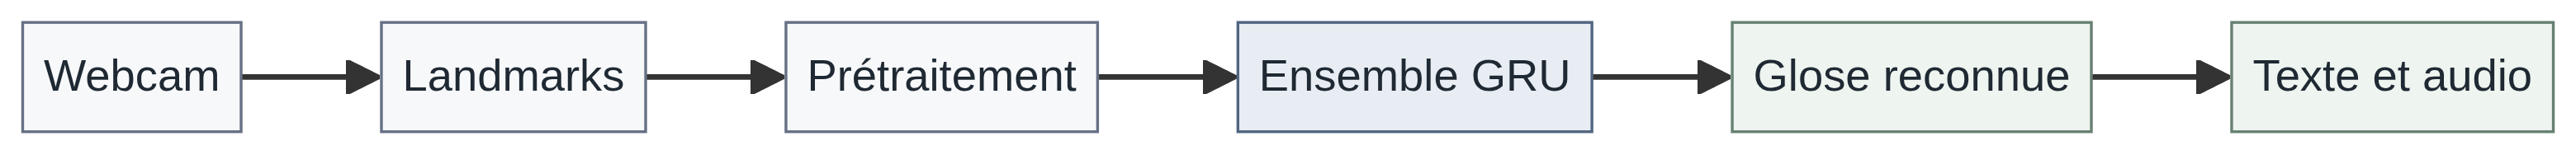
\includegraphics[width=0.90\textwidth,height=0.28\textheight,keepaspectratio]{figures/architecture_application_simple.png}
\caption{Chaîne essentielle de l'application : extraction des landmarks, prétraitement, classification par l'ensemble GRU et production d'une sortie textuelle ou audio.}
\label{fig:architecture-application}
\end{figure}

La Figure~\ref{fig:architecture-application} résume le chemin effectivement utilisé par l'interface. Les détails du contrat HTTP et les routes de comparaison sont présentés plus loin dans ce chapitre.

\section{Chaîne de données et traçabilité scientifique}

La chaîne de data science sépare les métadonnées, les séquences de landmarks, les transformations et les artefacts de modèles. Les partitions officielles et le manifeste d'intégrité sont conservés hors du dépôt public, tandis que les scripts de vérification, les configurations YAML, les métriques et les résumés sont versionnés. Le contrôle détecte les signeurs communs entre partitions, les identifiants dupliqués et les incompatibilités de forme avant l'entraînement.

Pour la phase GRU groupée, chaque exécution produit un résumé JSON, les prédictions et un checkpoint par fold. Les quinze checkpoints du modèle retenu sont conservés dans le registre des modèles. L'ensemble est agrégé par moyenne des probabilités pour l'évaluation et pour le mode actif de l'application. Le benchmark de latence distingue le temps de prédiction du modèle du temps de capture, de détection MediaPipe et de la synthèse vocale.

\section{Initialisation de la caméra et de MediaPipe}

L'utilisateur déclenche explicitement l'activation de la caméra. Le navigateur demande l'autorisation via l'API \texttt{getUserMedia}. MediaPipe Tasks Vision est ensuite chargé avec une version CDN documentée. Pose Landmarker et Hand Landmarker sont configurés en mode vidéo.

Pour chaque frame, le frontend récupère le premier résultat de pose et les résultats des mains. Une main non détectée est remplacée par 21 points nuls afin de conserver la forme de l'entrée. Cette stratégie garantit le contrat dimensionnel, mais elle ne garantit pas que l'information gestuelle soit suffisante. L'absence de mains doit donc rester visible dans l'analyse des erreurs.

\section{Capture et formation des fenêtres}

Le bouton de capture collecte 40 frames espacées d'environ 55 millisecondes. Trois fenêtres chevauchantes de 32 frames sont créées avec des débuts aux positions 0, 4 et 8. Chaque fenêtre respecte l'ordre des points défini par le contrat de prétraitement avant d'être envoyée au backend.

La méthode est volontairement cadrée. L'utilisateur réalise un signe isolé pendant la capture. Le système ne prétend pas détecter automatiquement une succession de signes dans une conversation. Cette décision réduit la complexité du démonstrateur et rend son comportement explicable.

\section{Guide d'utilisation de l'interface}

L'utilisation suit une séquence courte et déterministe. L'utilisateur clique d'abord sur « Activer la caméra » et autorise l'accès vidéo dans le navigateur. Le bouton « Analyser le signe » lance ensuite la capture d'une fenêtre de 40 frames. Le signe doit être réalisé seul, face à la caméra, dans un cadrage où les mains et le haut du corps restent visibles. Le système construit trois fenêtres chevauchantes, envoie les données à l'API et affiche les résultats classés.

La zone « Résultat » présente la meilleure glose, les trois hypothèses principales et leur score. Ce score est indicatif tant que la calibration GRU n'a pas été ajustée sur une validation hors échantillon. Le bouton « Écouter » lit le texte contrôlé associé à la prédiction ; il ne traduit pas une phrase LSFB et ne modifie pas la décision du modèle. Le bouton « Arrêter » désactive la caméra. Le bouton « Effacer » remet l'affichage à l'état initial. Une capture de l'état initial de l'interface est donnée à la Figure~\ref{fig:interface-application}.

\begin{figure}[ht]
\centering
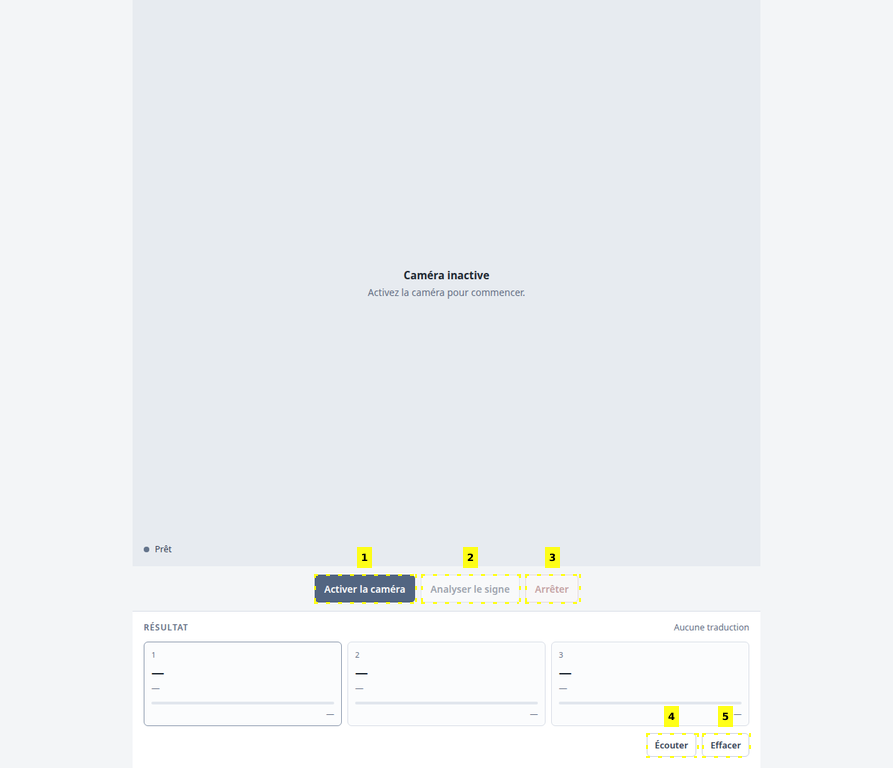
\includegraphics[width=0.62\textwidth]{figures/application_interface.png}
\caption{Interface du prototype : activation de la caméra, analyse d'un signe isolé, affichage du résultat et lecture vocale optionnelle.}
\label{fig:interface-application}
\end{figure}

Cette procédure limite les erreurs d'usage, mais elle ne constitue pas encore un protocole de traduction en visioconférence. Une application continue devra afficher l'état de la segmentation, distinguer une hypothèse temporaire d'une sortie confirmée et permettre de corriger ou d'annuler une phrase avant sa vocalisation.

\section{Contrat HTTP}

La route active \texttt{POST /predict-gru} attend un objet JSON contenant \texttt{landmarks}. La matrice reçue doit avoir exactement 32 lignes et 225 valeurs par ligne. Elle correspond aux 33 points de pose et aux 42 points de mains en trois coordonnées. L'API convertit les données en tableau NumPy, vérifie la forme et rejette les valeurs non finies.

Le backend normalise ensuite chaque frame par rapport au torse et ajoute les deux poignets relatifs au torse. La représentation interne contient 231 valeurs par frame. Les quinze GRU produisent des distributions softmax qui sont moyennées avant le classement final. La réponse conserve le score brut, le score calibré lorsqu'un artefact de calibration validé existe, la marge entre les deux premières classes et l'accord des quinze réseaux.

La réponse contient la glose prédite, sa confiance, les trois meilleurs résultats, le temps d'inférence, la version du modèle et la représentation utilisée. Elle indique aussi \texttt{confidence\_calibrated}, \texttt{raw\_confidence}, \texttt{margin}, \texttt{ensemble\_agreement}, \texttt{accepted} et \texttt{rejection\_reason}. Tant qu'une calibration apprise sur validation groupée n'est pas installée, \texttt{accepted} vaut \texttt{null} et aucun rejet scientifique n'est déclaré. Les routes \texttt{/health} et \texttt{/model-info} servent respectivement au diagnostic et à l'inspection des métadonnées de l'ensemble actif.

Le Tableau~\ref{tab:contrats-http} récapitule les routes actives, historiques et de comparaison ainsi que leurs formes d'entrée.

\begin{table}[ht]
\centering
\small
\caption{Contrats HTTP du prototype et statut de chaque route.}
\label{tab:contrats-http}
\begin{tabular}{p{4.3cm}p{2.5cm}p{9.4cm}}
\hline
Route & Entrée principale & Fonction et statut \\
\hline
\texttt{/health} & Aucune & État du service, modèle actif et nombre de checkpoints \\
\texttt{/model-info} & Aucune & Métadonnées de l'ensemble GRU retenu actif \\
\texttt{/candidate-info} & Aucune & Métadonnées du RF historique conservé pour le repli \\
\texttt{/predict-gru} & \texttt{[32,225]} & Route finale de l'interface web \\
\texttt{/predict} & \texttt{[32,225]} & Route baseline conservée pour les tests \\
\texttt{/predict-candidate} & \texttt{[32,126]} & Route RF historique conservée pour comparaison \\
\hline
\end{tabular}
\end{table}

La route \texttt{/predict-gru} est la seule route de prédiction utilisée par l'interface finale. Les autres routes restent accessibles pour la traçabilité, la comparaison et le retour arrière, mais ne sont pas proposées comme choix à l'utilisateur.

\section{Stabilisation de la décision}

Le classement et le rejet sont deux décisions distinctes. La future règle de rejet combinera le score calibré, la marge top-1--top-2 et l'accord des quinze réseaux. Les seuils seront appris sur une validation groupée par signeur en optimisant le risque à couverture fixée ; ils ne seront pas choisis à partir du test officiel. Dans l'état courant, la calibration n'est pas encore installée, l'interface affiche le top-3 et le statut « score non calibré », et la vocalisation reste désactivée sous le seuil d'interface historique de 55 pour cent.

La stabilisation agit au niveau de l'interface. Elle ne modifie pas les paramètres du classifieur et ne transforme pas une mauvaise prédiction en bonne prédiction. Elle constitue une règle de décision applicative et non une amélioration mesurée du modèle. Une calibration future ne changera pas le classement top-1 ; elle rendra seulement le niveau de confiance et le rejet plus interprétables.

\section{Génération du texte et synthèse vocale}

Une table JavaScript associe chaque classe à un texte français contrôlé. Le texte est affiché après validation de la stabilité. La Web Speech API crée automatiquement une utterance vocale pour la meilleure prédiction stable, c'est-à-dire la classe retenue par le modèle lorsque le seuil de confiance applicatif est atteint \cite{WebSpeech}. Un bouton secondaire permet uniquement de répéter le dernier résultat. La logique annule une vocalisation précédente avant d'en lancer une nouvelle et mémorise la dernière décision prononcée afin d'éviter les répétitions.

Le modèle produit une classe de glose. La table de sortie lui associe un texte contrôlé. Le navigateur produit ensuite le son. La qualité de la voix dépend du navigateur et des voix installées ; elle doit être documentée comme une propriété de la couche de présentation et non comme une performance de reconnaissance LSFB.

Un mode expérimental peut enchaîner des segments causaux et conserver une liste de gloses. Cette liste constitue une étape vers la transcription visuelle de séquences, mais elle ne doit pas être appelée transcription continue validée sans corpus comportant des séquences annotées, des frontières temporelles et une mesure par distance d'édition.

\section{Gestion des erreurs et sécurité du contrat}

L'API refuse les entrées de forme incorrecte et les valeurs non finies. Au démarrage, elle vérifie la correspondance entre les classes, le nombre de caractéristiques et les métadonnées de configuration. Ces contrôles empêchent de charger silencieusement un modèle incompatible avec le frontend.

Les tests automatisés couvrent le healthcheck, les métadonnées, une prédiction GRU valide, une forme incorrecte et une valeur non finie. Le test de robustesse sur 5\,957 séquences confirme également le rejet de trois payloads invalides par le code HTTP 422. Ces contrôles ne remplacent pas un test navigateur, mais ils garantissent le contrat backend minimal.

\section{Migration intermédiaire vers le Random Forest mains seules}

Une migration intermédiaire vers \texttt{wrist\_scaled} a d'abord été réalisée pour réduire la dimension de l'entrée et vérifier la cohérence entre le frontend et un modèle RF. Le frontend conservait alors les 42 points des deux mains, appliquait le même centrage et la même échelle que le script d'entraînement et utilisait \texttt{/predict-candidate} avec une entrée \texttt{[32,126]}. L'ancien contrat pose--mains \texttt{[32,225]} et la baseline historique ont été conservés pour les tests et le retour arrière.

Cette étape RF a été utile comme champion intermédiaire. Elle a toutefois été dépassée par l'évaluation groupée des modèles GRU, qui a apporté un gain sur le test officiel dans le protocole final. La migration RF reste documentée afin de rendre la chronologie reproductible.

\section{Bascule finale vers l'ensemble GRU retenu}

La bascule finale a remplacé le contrat actif par \texttt{/predict-gru}. Le frontend transmet les landmarks de pose et des mains sous la forme \texttt{[32,225]}. Le backend applique la normalisation par le torse, ajoute les poignets relatifs et exécute les quinze checkpoints du modèle retenu. Les artefacts, leurs manifestes et les tests sont conservés dans GitHub.

La décision d'activer la GRU repose sur deux niveaux de preuve. La comparaison finale sur le test officiel donne une accuracy de 82,31 pour cent et un macro-F1 de 0,8153. Le test API indépendant de l'implémentation hors ligne, réalisé sur les 5\,957 mêmes séquences, reproduit ces métriques. La GRU est donc le modèle actif dans le périmètre étudié, tandis que le RF reste une solution de comparaison et de repli.

\section{Tests d'inférence et mesure de latence}

Un benchmark synthétique de la route \texttt{/predict-gru} a mesuré une moyenne HTTP de 68,19 millisecondes sur 10 appels. Le test de robustesse sur le split officiel a mesuré une moyenne de 63,59 millisecondes, une médiane de 59,57 millisecondes, un P95 de 86,79 millisecondes et un P99 de 109,41 millisecondes par séquence.

Ces chiffres caractérisent le trajet HTTP et l'inférence GRU sur des landmarks déjà extraits. Ils n'incluent pas l'acquisition de la caméra, l'extraction MediaPipe, la consolidation complète des fenêtres ni la synthèse vocale. La mesure de la chaîne complète nécessite un protocole de capture dédié sur un poste équipé.

\section{Portée de la notion de temps réel}

L'application actuelle fonctionne par fenêtres : elle capture 40 images, construit trois fenêtres de 32 frames, attend la fin de la capture, puis envoie les fenêtres au backend et consolide les réponses. Le prototype fournit ainsi une interaction rapide après une capture, mais il ne réalise pas une traduction continue frame par frame.

Le système actuel fonctionne comme une reconnaissance interactive de gloses LSFB isolées par fenêtres, avec sortie textuelle contrôlée et synthèse vocale optionnelle après capture. La reconnaissance continue demanderait une acquisition en continu, une segmentation causale validée, une mesure de latence de bout en bout, un corpus de séquences annotées et une évaluation sur vidéo réelle.

\section{Conclusion du chapitre}

Ce chapitre a décrit l'architecture finale du prototype. La capture, l'extraction des landmarks, le prétraitement GRU, l'inférence de l'ensemble configuration GRU retenue, la stabilisation et la synthèse vocale sont séparés par des contrats vérifiables. L'application fournit une reconnaissance interactive de gloses isolées ; le RF est conservé pour le repli, tandis que la traduction continue reste hors du périmètre démontré.

Le chapitre suivant discute les performances, les erreurs résiduelles, les limites de l'évaluation API et les perspectives nécessaires pour passer d'une reconnaissance isolée à une chaîne webcam complète.

\chapter{Évaluation des modèles et résultats}

\section{Objectif et organisation de l'évaluation}

Ce chapitre évalue la capacité du système à reconnaître douze gloses LSFB isolées à partir de landmarks. L'objectif n'est pas de mesurer une traduction ouverte de phrases, mais de comparer des représentations et des classifieurs dans un protocole contrôlé, puis d'identifier la configuration retenue pour l'application web.

Les expériences utilisent les splits officiels de LSFB-ISOL. Les signeurs de test ne sont pas utilisés pour l'entraînement. Lorsque cela est indiqué, chaque classe est limitée à 100 séquences d'entraînement et 50 séquences de test. Les métriques principales sont l'accuracy, le macro-F1 et la balanced accuracy. Le macro-F1 est privilégié pour éviter qu'une bonne performance sur quelques classes masque des classes moins bien reconnues.

Le chapitre distingue les performances du classifieur et les contrôles d'intégration. Les détails du contrat HTTP et des endpoints sont définis dans le chapitre consacré à l'application ; ici, le test d'intégration est utilisé uniquement pour vérifier que le modèle gelé est reproduit sans modification lors du déploiement.

\section{Protocole scientifique et gel de la configuration GRU retenue}

Le protocole final a été gelé avant la comparaison du test officiel. Il utilise le vocabulaire contrôlé de douze gloses, les 7\,590 séquences d'entraînement autorisées et les 5\,957 séquences du test officiel. La séparation est faite par signeur : les 59 signeurs d'entraînement et les 40 signeurs de test ne se recouvrent pas. Les doublons d'identifiants et les doublons de lignes sont contrôlés avant l'entraînement.

La validation interne utilise trois graines, 7, 42 et 101, et cinq folds stratifiés groupés par signeur. Chaque checkpoint est sélectionné uniquement sur la validation de son fold avec le macro-F1. Les données de validation ne sont pas mélangées avec les données d'entraînement et le test officiel n'est pas utilisé pour régler les hyperparamètres, les représentations ou l'arrêt précoce.

La configuration GRU retenue reprend le protocole d'GRU initiale et ajoute uniquement les deux poignets relatifs au centre des épaules. Les autres éléments sont conservés : corpus, classes, graines, folds, longueur de 32 frames, architecture GRU et règle d'optimisation. Cette contrainte permet d'interpréter l'expérience comme une ablation ciblée de la représentation, même si la comparaison finale avec le RF reste une comparaison de configurations complètes.

Le modèle est gelé pour trois raisons. Premièrement, configuration GRU retenue obtient le meilleur macro-F1 de validation moyen parmi les configurations GRU comparées, avec 0,7326 et un écart-type de 0,0309. Deuxièmement, il améliore le résultat de test d'GRU initiale, de 0,8130 à 0,8153 en macro-F1, avec une balanced accuracy de 0,8129. Troisièmement, les quinze checkpoints, leurs manifestes et les tests API sont archivés et reproduisent le contrat d'inférence. Le gain est faible ; le gel ne signifie donc pas que la supériorité est définitivement prouvée. Il signifie que la configuration est figée pour éviter de modifier le modèle après consultation du test.

Après le gel, aucune modification de poids, de classes, de prétraitement ou de seuil de décision n'est appliquée pour améliorer le score du test officiel. Toute calibration de confiance ou politique de rejet future devra être apprise sur une validation séparée et enregistrée comme une nouvelle étape, sans réécrire les résultats de la configuration GRU retenue.

\section{Synthèse des études récentes}

Les premières expériences du projet ont servi à vérifier la faisabilité du pipeline et à comparer quelques représentations sur des sous-échantillons limités. Elles sont conservées dans les journaux expérimentaux et les annexes, mais elles ne constituent pas le résultat principal du mémoire. La suite de l'analyse porte sur les expériences récentes, conduites sur les partitions officielles et avec une validation groupée par signeur lorsque cela est possible.

\begin{table}[ht]
\centering
\small
\caption{Succession des configurations dans la stratégie champion/challenger.}
\label{tab:champion-challenger}
\begin{tabular}{p{3.2cm}p{3.3cm}p{5.0cm}p{3.8cm}}
\hline
Configuration & Représentation & Rôle dans la sélection & Statut final \\
\hline
RF plafonné & \texttt{raw}/\texttt{wrist\_scaled} & Baseline exploratoire sur corpus limité & Écarté \\
Random Forest complet & \texttt{wrist\_scaled} séquence complète & Challenger RF avec toutes les séquences d'entraînement & Référence et repli \\
GRU initiale & Pose--mains normalisées & Challenger temporel groupé par signeur & Dépassé par configuration GRU retenue \\
GRU retenue avec poignets relatifs & Pose--mains + poignets relatifs & Ablation finale et test API de robustesse & Modèle actif \\
\hline
\end{tabular}
\end{table}

Le Tableau~\ref{tab:champion-challenger} distingue les résultats exploratoires des décisions finales. Les chiffres du test officiel sont utilisés uniquement pour comparer les candidats gelés ; les représentations et les hyperparamètres sont réglés sur la validation groupée.

La Figure~\ref{fig:revision-boxplot} présente la dispersion des scores de validation des quinze folds GRU. Le Random Forest complet est affiché comme une référence ponctuelle du test verrouillé, car son artefact complet ne fournit pas une distribution de folds directement comparable à celle des GRU.

\begin{figure}[ht]
\centering
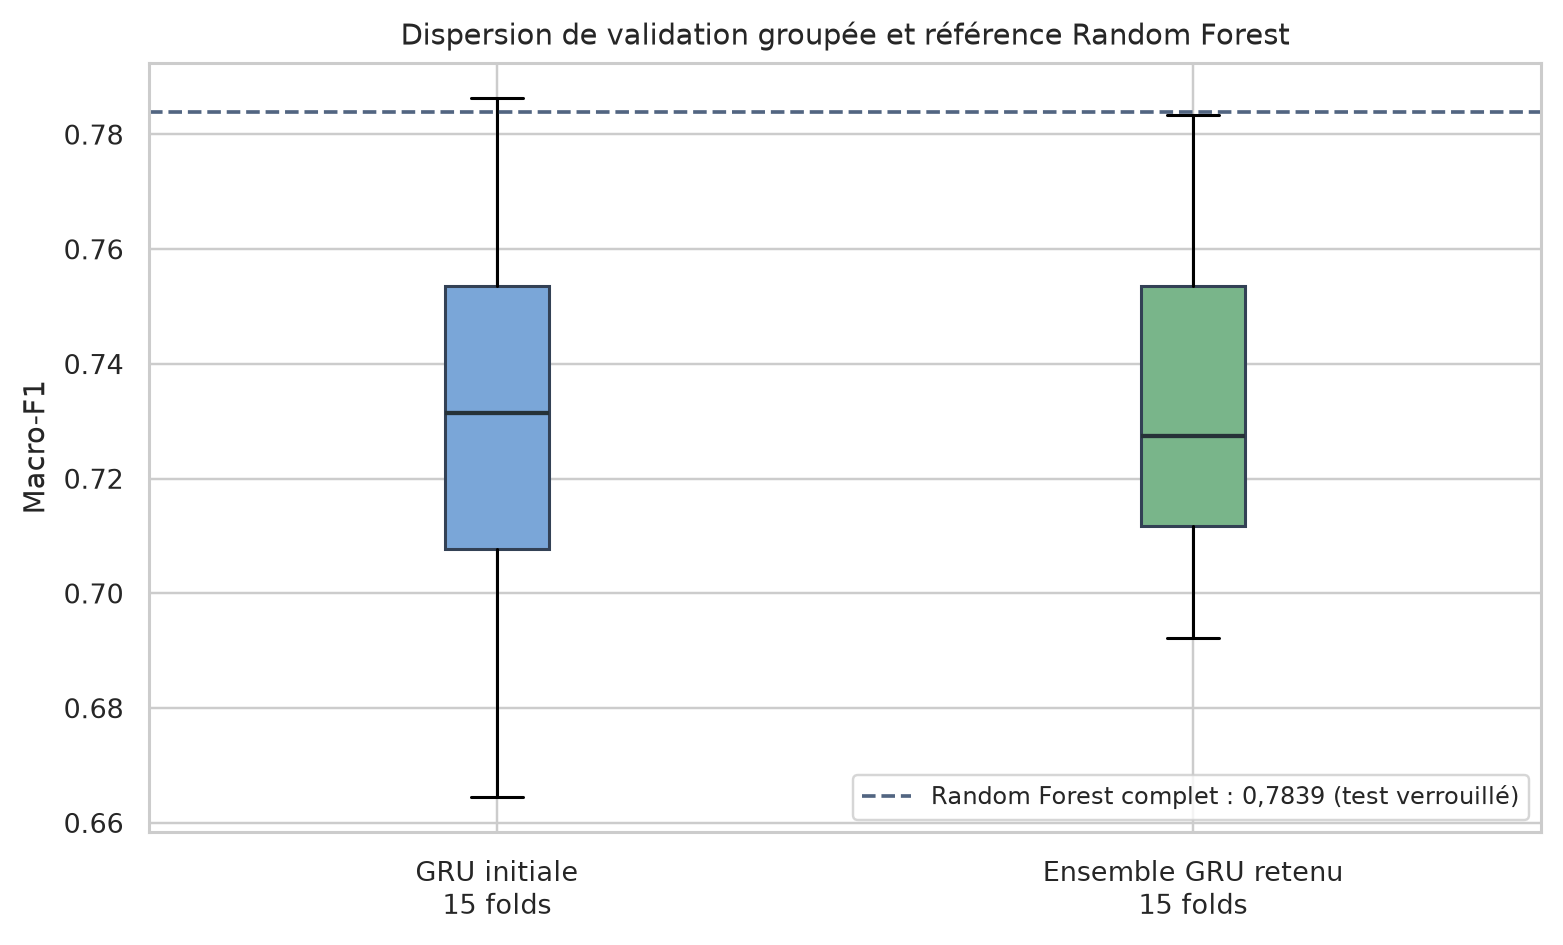
\includegraphics[width=0.94\textwidth]{figures/generated/revision_boxplot_macro_f1_gru_rf.png}
\caption{Dispersion du macro-F1 sur les folds groupés des GRU initiale et configuration GRU retenue ; la ligne pointillée indique le score de test verrouillé du Random Forest complet.}
\label{fig:revision-boxplot}
\end{figure}

\subsection{GRU initiale : validation groupée de la GRU}

GRU initiale évalue une GRU bidirectionnelle compacte avec 32 frames, trois graines (7, 42 et 101) et cinq folds groupés par signeur. Les signeurs de validation restent donc séparés des signeurs utilisés pour l'entraînement. Les quinze checkpoints atteignent un macro-F1 de validation moyen de 0,7297, avec un écart-type d'échantillon de 0,0344. Sur le test officiel verrouillé de 5\,957 séquences, l'agrégation des quinze modèles atteint une accuracy de 82,21\,%, un macro-F1 de 0,8130 et une balanced accuracy de 0,8099.

Ce résultat établit la GRU comme le meilleur candidat expérimental avant l'ablation suivante. Il doit cependant être interprété comme le résultat d'un ensemble de quinze checkpoints, et non comme la performance d'une GRU unique. La dispersion du macro-F1 par signeur reste importante : elle montre que la généralisation dépend encore des caractéristiques des signeurs et des conditions de capture.

\subsection{configuration GRU retenue : ablation des poignets relatifs au torse}

La configuration GRU retenue ajoute aux landmarks pose--mains les positions des deux poignets relatives au centre des épaules. Le corpus, les graines, les folds et les hyperparamètres restent inchangés par rapport à GRU initiale. Le macro-F1 moyen de validation progresse de 0,7297 à 0,7326, tandis que l'écart-type passe de 0,0338 à 0,0309. Sur le test officiel, l'accuracy progresse de 82,21\,% à 82,31\,%, le macro-F1 de 0,8130 à 0,8153 et la balanced accuracy de 0,8099 à 0,8129.

L'analyse par classe nuance ce gain global. Les améliorations les plus importantes concernent SOURD (+0,0258 de F1), COMPRENDRE (+0,0180), NON (+0,0166) et REGARDER (+0,0117). En revanche, BIEN (-0,0190), QUOI (-0,0130), DIRE (-0,0128) et AVOIR (-0,0125) se dégradent. La confusion NON vers SOURD diminue de 87 à 68 occurrences et la confusion FINIR vers OUI diminue de 56 à 50. À l'inverse, la confusion AVOIR vers QUOI augmente de 36 à 49 occurrences. L'ajout des poignets améliore donc certaines ambiguïtés spatiales sans résoudre toutes les confusions gestuelles.

Le gain de 0,0023 de macro-F1 sur le test est faible. configuration GRU retenue est ainsi conservée comme meilleure configuration observée, mais elle ne doit pas être présentée comme une amélioration définitivement robuste avant une réplication sur de nouvelles partitions de signeurs.

\subsection{Random Forest complet et calibration}

Le Random Forest complet réentraîne le Random Forest avec l'ensemble des 7\,590 séquences d'entraînement, au lieu du plafond historique de 100 séquences par classe. Pour permettre une comparaison correcte avec configuration GRU retenue, le protocole retenu rééchantillonne chaque séquence complète sur 32 frames, puis applique \texttt{wrist\_scaled} aux deux mains. L'entrée possède la forme \texttt{[32,126]} avant aplatissement. Le classifieur utilise 300 arbres et des poids équilibrés. Le paramètre \texttt{max\_features} vaut \texttt{sqrt}, avec une graine fixée à 42.

Sur les mêmes 5\,957 séquences de test, le RF complet atteint une accuracy de 79,03\,%, un macro-F1 de 0,7839 et une balanced accuracy de 0,7931. Il améliore donc nettement les anciennes baselines limitées, mais reste inférieur à l'ensemble GRU retenu. Le premier essai causal d'Random Forest complet, qui segmentait les séquences avant le rééchantillonnage, n'atteignait que 73,14\,% d'accuracy. Cette différence montre que la segmentation causale et la classification hors ligne ne doivent pas être confondues.

La calibration isotonic réduit l'Expected Calibration Error du RF de 0,2124 à 0,0455 et le Brier score de 0,3665 à 0,3037. Elle rend les scores plus interprétables comme niveaux de confiance, mais diminue légèrement l'accuracy de 79,03\,% à 78,73\,% et le macro-F1 de 0,7839 à 0,7801. Le modèle calibré est donc utile pour une politique de rejet, mais ne doit pas être activé uniquement pour maximiser la classification.

La Figure~\ref{fig:revision-reliability} complète ces métriques par un diagramme de fiabilité. Les courbes restent éloignées de la diagonale pour le RF brut, tandis que la calibration isotonic redistribue les niveaux de confiance. Cette figure concerne le RF. La GRU active expose désormais séparément son score brut, sa marge et l'accord des quinze réseaux, mais son artefact de température n'est pas encore produit : les scores GRU restent donc explicitement non calibrés.

\begin{figure}[ht]
\centering
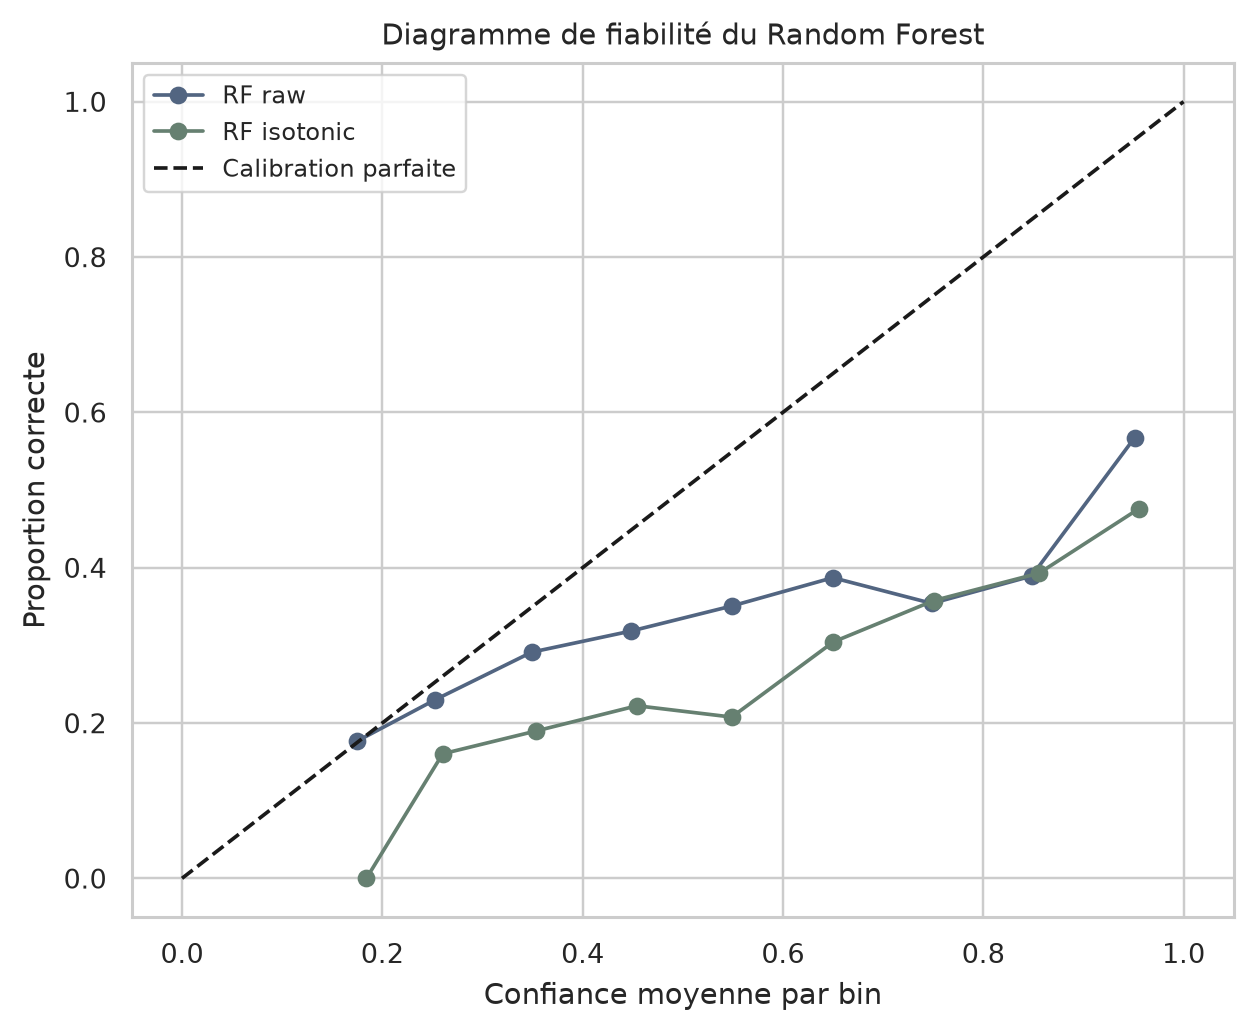
\includegraphics[width=0.90\textwidth]{figures/generated/revision_reliability_rf.png}
\caption{Diagramme de fiabilité du Random Forest complet avant et après calibration isotonic sur le test officiel.}
\label{fig:revision-reliability}
\end{figure}

\subsection{Comparaison récente et décision}

Le tableau suivant rassemble les résultats qui doivent être retenus dans la discussion du mémoire. Les anciennes expériences servent uniquement à documenter la progression du projet ; elles ne doivent pas être utilisées pour comparer directement les modèles récents, car leurs tailles de corpus, représentations et règles de fenêtrage diffèrent.

Le Tableau~\ref{tab:recent-results-summary} donne les métriques principales, et le Tableau~\ref{tab:gru-api-per-class} détaille la robustesse de l'ensemble GRU par glose.

\begin{table}[ht]
\centering
\small
\caption{Résultats récents sur le test officiel de 5\,957 séquences.}
\label{tab:recent-results-summary}
\begin{tabular}{lccc}
\hline
Configuration & Accuracy & Macro-F1 & Balanced accuracy \\
\hline
Random Forest complet & 79,03\,\% & 0,7839 & 0,7931 \\
RF calibré isotonic & 78,73\,\% & 0,7801 & 0,7853 \\
GRU initiale, 15 checkpoints & 82,21\,\% & 0,8130 & 0,8099 \\
GRU retenue avec poignets relatifs, 15 checkpoints & \textbf{82,31\,\%} & \textbf{0,8153} & \textbf{0,8129} \\
\hline
\end{tabular}
\end{table}

La Figure~\ref{fig:revision-class-bars} met en évidence les différences par glose. Le gain de la GRU n'est pas uniforme : il est particulièrement visible pour DIFFERENT, OUI et SOURD, tandis que certaines classes comme QUOI restent proches du RF et que les confusions FINIR ou NON demeurent difficiles. Les classes NON et SOURD sont surlignées, car leur séparation reste un point de diagnostic important.

\begin{figure}[ht]
\centering
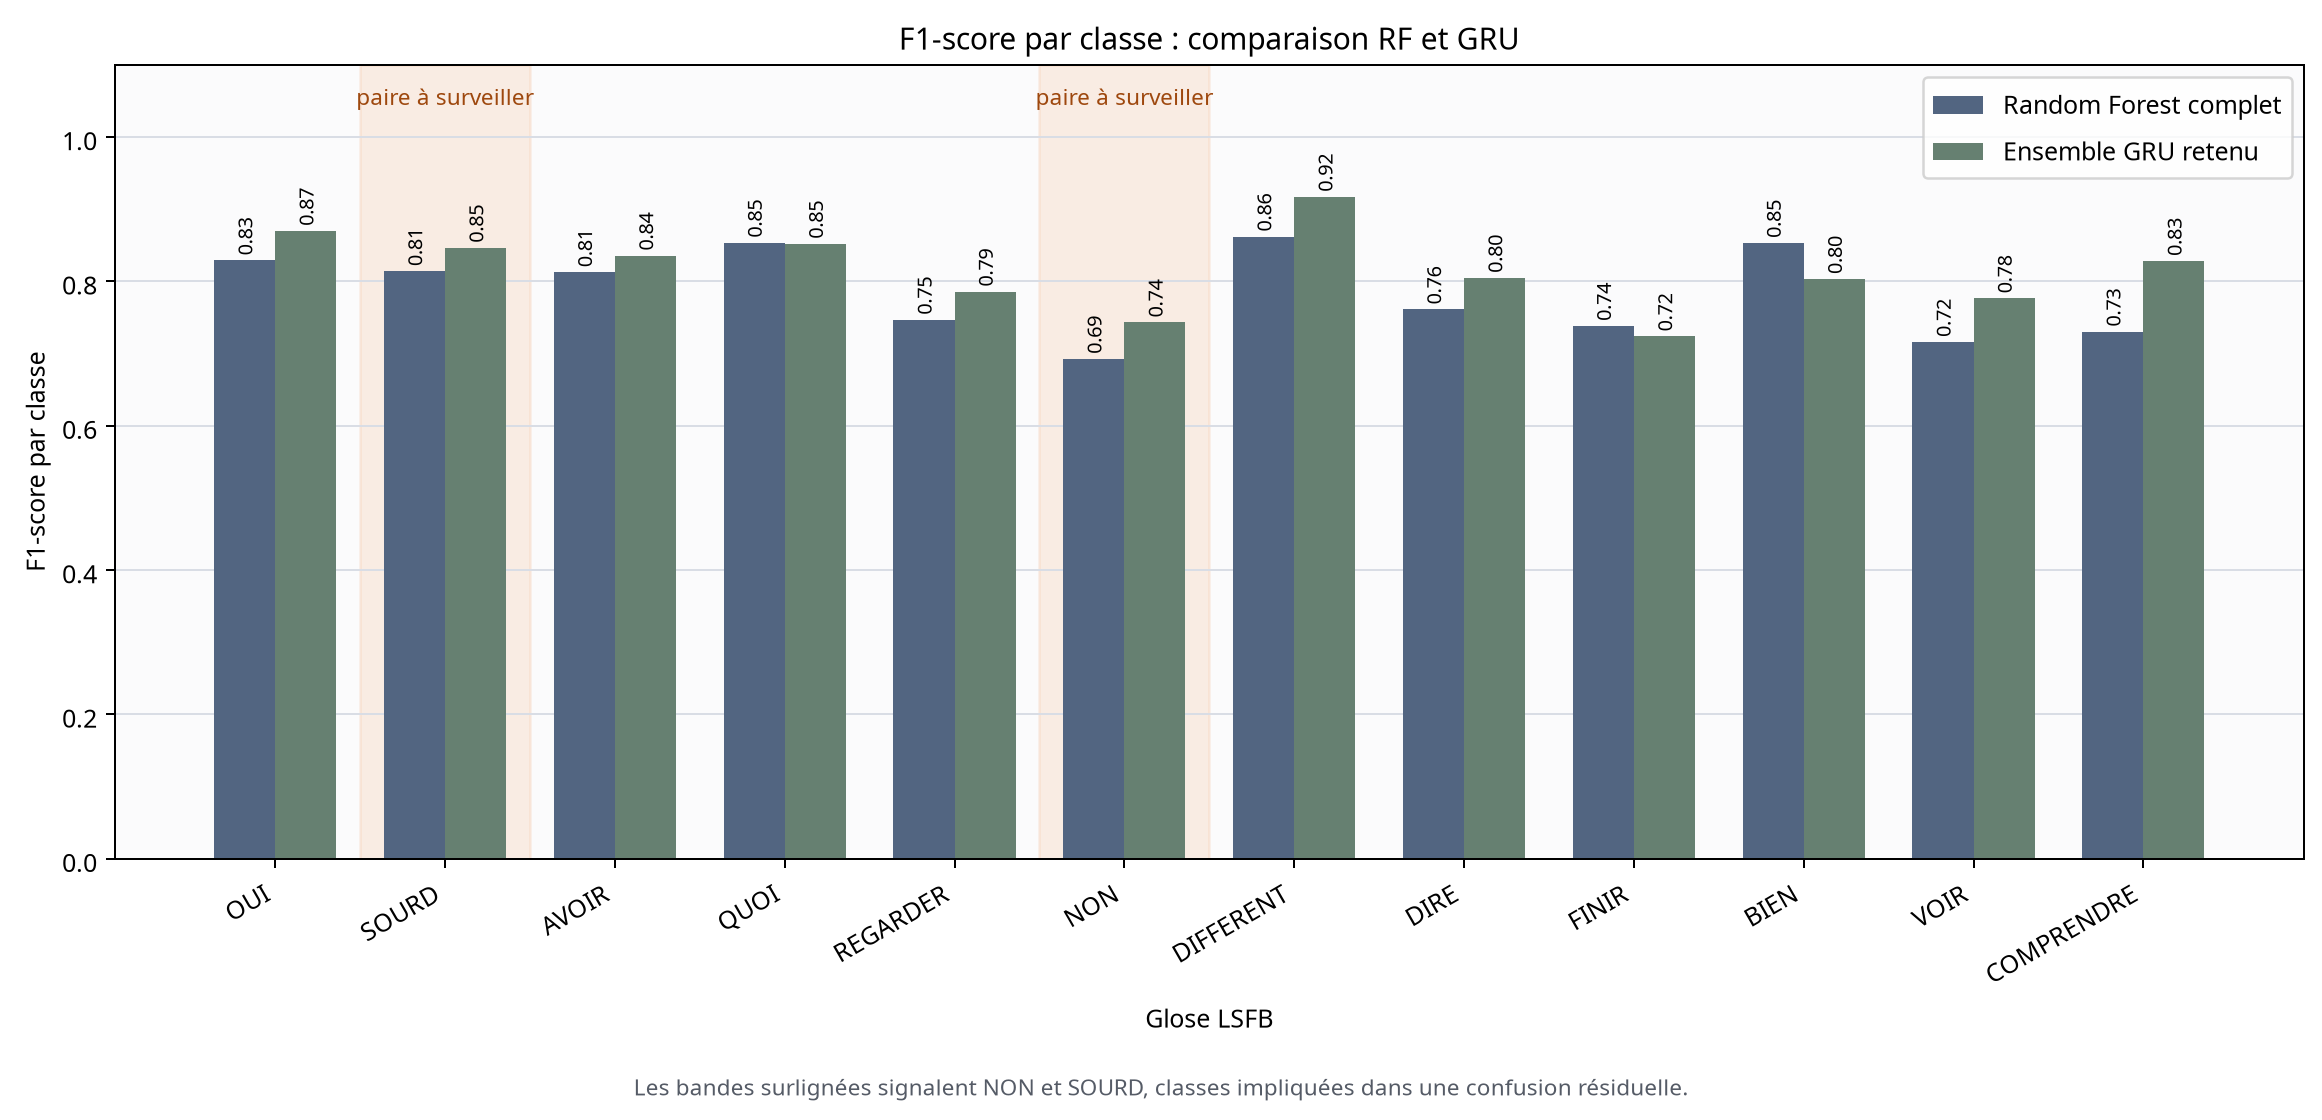
\includegraphics[width=0.98\textwidth]{figures/generated/f1_par_classe_gru_rf_non_sourd.png}
\caption{F1-score par classe entre le Random Forest complet et l'ensemble GRU retenu sur le test officiel. Les bandes indiquent NON et SOURD.}
\label{fig:revision-class-bars}
\end{figure}

L'ensemble GRU retenu constitue le meilleur résultat expérimental observé et devient également le modèle actif de l'application. Le RF complet reste conservé pour les comparaisons et le retour arrière. Cette décision est fondée sur le gain mesuré sur le test officiel et sur la vérification du contrat d'inférence, tout en conservant une surveillance de la latence.

\subsection{Pistes d'amélioration fondées sur les résultats récents}

La prochaine amélioration prioritaire consiste à comparer RF et GRU avec la même représentation, les mêmes folds et les mêmes règles de segmentation. Cette expérience permettra de distinguer l'effet de l'architecture de celui de l'information pose--mains et des poignets relatifs au torse. Elle doit précéder toute conclusion sur la supériorité intrinsèque de la GRU.

Pour le RF, une recherche groupée d'hyperparamètres peut comparer le nombre d'arbres, la profondeur maximale, la taille minimale des feuilles et \texttt{max\_features}, sans consulter le test officiel pendant la sélection. Pour la GRU, les pistes les plus prometteuses sont l'entraînement d'un modèle unique, la distillation de l'ensemble de quinze checkpoints et la comparaison de fenêtres de 16, 24, 32 et 48 frames. Ces variantes ne seront retenues que si elles préservent le macro-F1 des classes difficiles et le pire signeur.

L'analyse configuration GRU retenue indique aussi une priorité linguistique et géométrique : réduire les confusions AVOIR--QUOI sans perdre les gains obtenus sur NON--SOURD. Une analyse des landmarks manquants, des vitesses et des angles peut être conduite dans les folds d'entraînement. Enfin, la calibration GRU doit être ajustée sur des prédictions hors-échantillon de validation groupée par signeur. La température sera apprise par minimisation de la log-vraisemblance, puis les seuils de confiance, de marge et d'accord seront choisis sur une courbe risque--couverture avec une couverture cible fixée avant l'évaluation finale. Les intervalles seront bootstrapés au niveau du signeur. Le test officiel restera réservé à la mesure finale et ne servira ni à apprendre la température ni à choisir les seuils. Une prédiction « incertaine » est préférable à une confiance élevée mais mal calibrée, mais elle ne sera rejetée que selon cette procédure pré-enregistrée.

\section{Choix du modèle et validation applicative}

Le modèle retenu pour l'interface est l'ensemble GRU retenu, composé de quinze checkpoints. Le frontend transmet 33 landmarks de pose et 42 landmarks de mains, soit une entrée brute de forme \texttt{[32,225]}. L'API normalise chaque séquence par rapport au torse, ajoute les deux poignets relatifs au torse et produit la représentation interne \texttt{[32,231]}. Le Random Forest complet et le candidat RF historique restent versionnés pour la comparaison et le retour arrière.

Les tests automatisés vérifient les contrats HTTP, la forme des matrices, la cohérence des labels, le classement top-3 et le chargement des quinze checkpoints. La route active est \texttt{/predict-gru}. Un benchmark synthétique séparé de 10 appels a mesuré une moyenne HTTP de 68,19 millisecondes et un P95 de 119,19 millisecondes. Cette mesure sert de contrôle de service et exclut la webcam, MediaPipe et la synthèse vocale.

La Figure~\ref{fig:benchmark-latence} représente les moyennes et les étendues min--max de ce benchmark contractuel. Elle doit être lue comme une mesure du service HTTP sur des matrices synthétiques valides, et non comme une mesure de latence utilisateur de bout en bout.

\begin{figure}[ht]
\centering
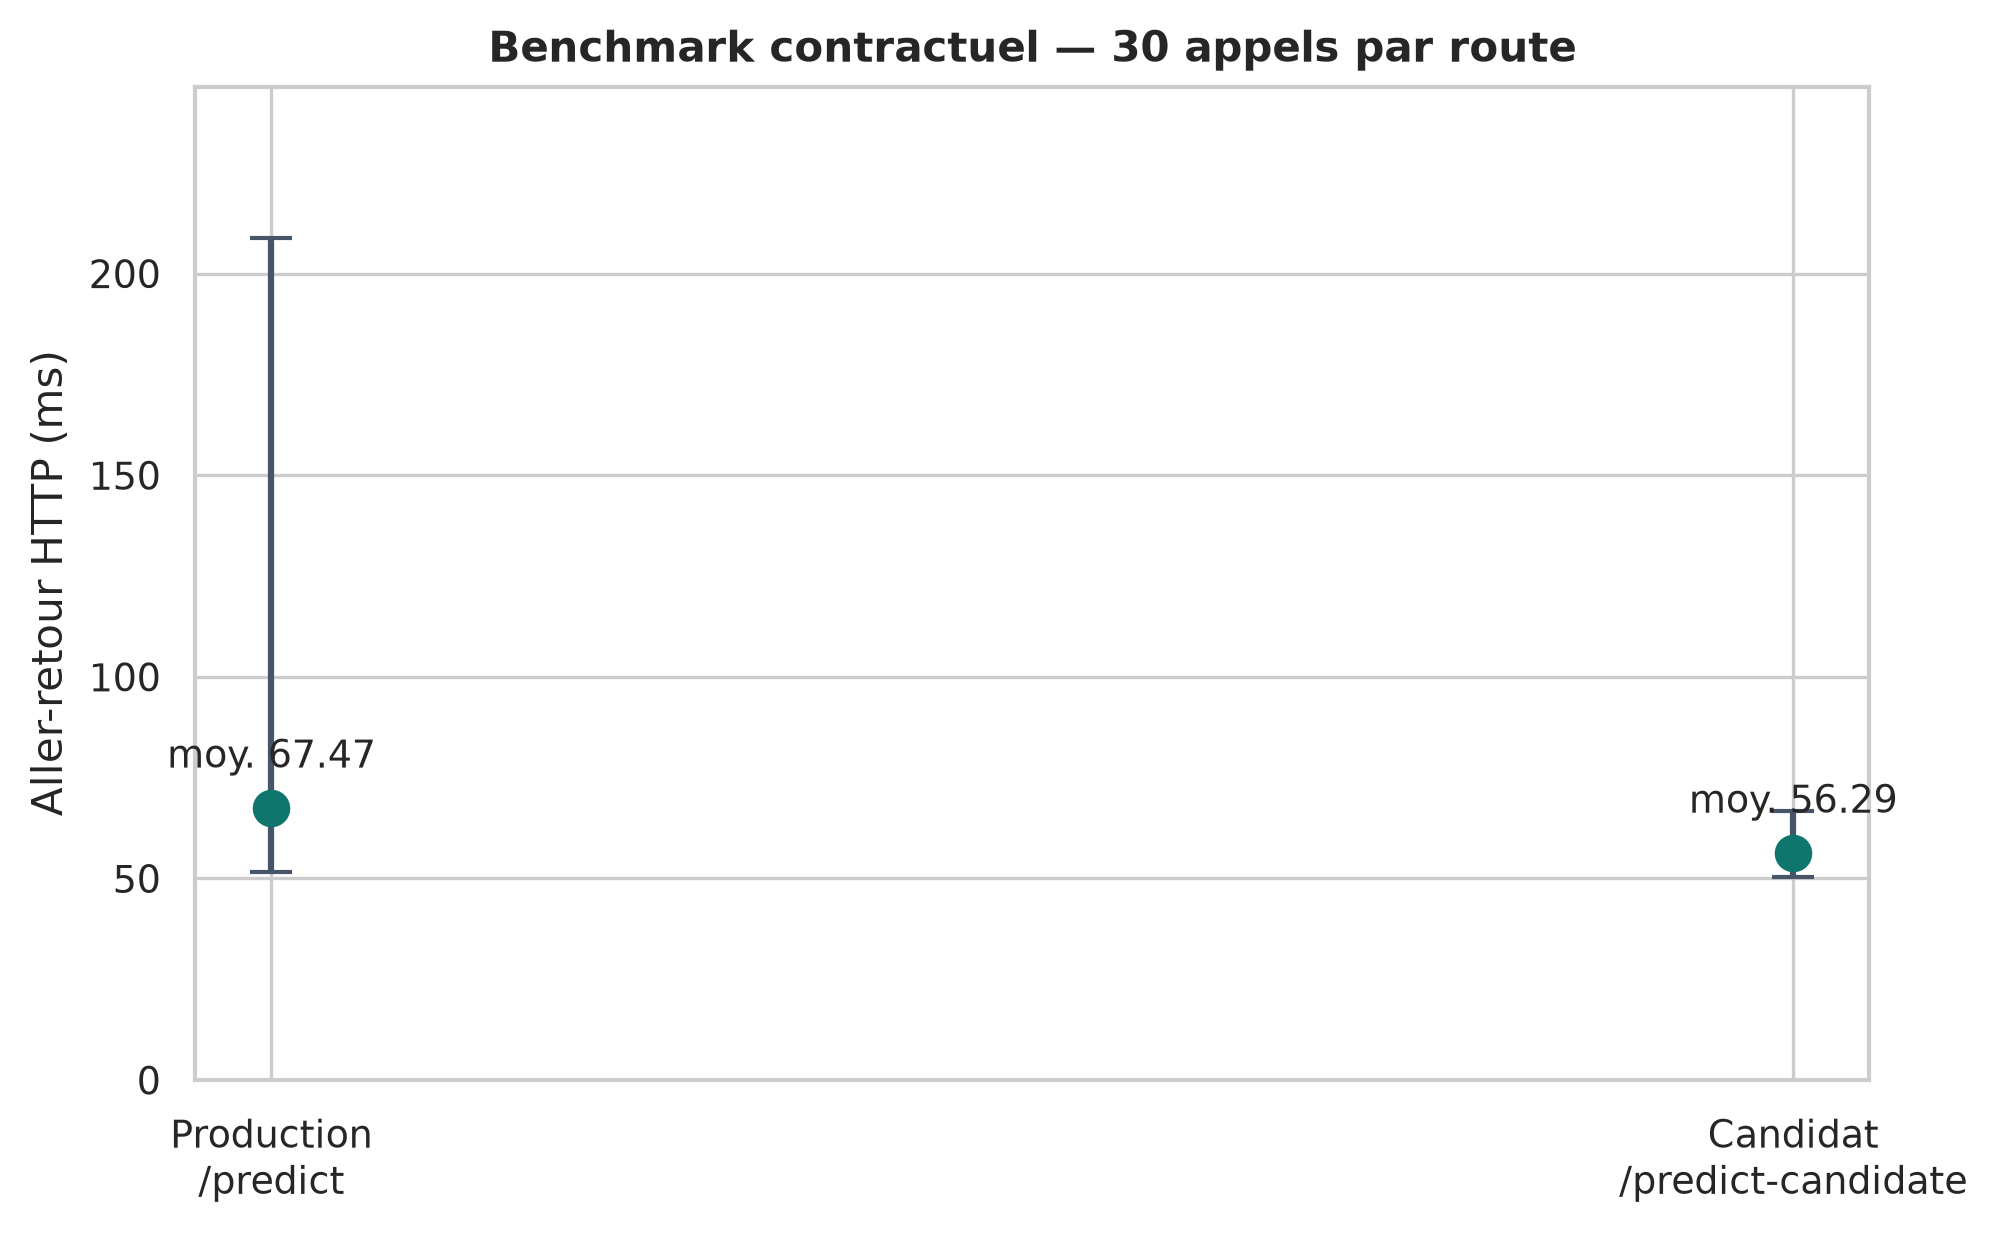
\includegraphics[width=0.94\textwidth]{figures/generated/benchmark_api_latency.png}
\caption{Latence d'aller-retour HTTP des routes de prédiction sur 30 appels contractuels.}
\label{fig:benchmark-latence}
\end{figure}

La validation ci-dessus porte sur le classifieur et l'API. Elle ne mesure pas encore le temps d'extraction MediaPipe ni la synthèse vocale. Le résultat applicatif doit donc être décrit comme une reconnaissance interactive par fenêtres, et non comme une traduction continue en temps réel.

\section{Limites et validité des conclusions}

Les résultats portent sur douze gloses isolées, des landmarks déjà extraits et un corpus contrôlé. Ils ne mesurent pas la traduction de phrases, la syntaxe LSFB, la reconnaissance de plusieurs signes successifs ni la qualité linguistique d'une sortie française.

Les performances dépendent de la qualité de MediaPipe, de l'éclairage, du cadrage, de la morphologie, de la vitesse d'exécution et des signeurs. Les cinq graines donnent une estimation utile de la variabilité, mais ne constituent pas une caractérisation exhaustive de l'incertitude. Les mesures API synthétiques ne remplacent pas un test webcam équipé et annoté.

Sur les 240 séquences isolées disponibles pour la validation exploratoire de la machine à états, une activité est détectée dans 75,4\,\% des cas et un repli ou une absence de détection est observé dans 24,6\,\% des cas. La Figure~\ref{fig:causal-detection} résume ce résultat. Les faux départs et les signes manqués ne sont pas estimables avec un corpus de signes isolés sans frontières annotées dans un flux continu ; aucune précision de segmentation ne doit donc être déduite de cette proportion.

\begin{figure}[ht]
\centering
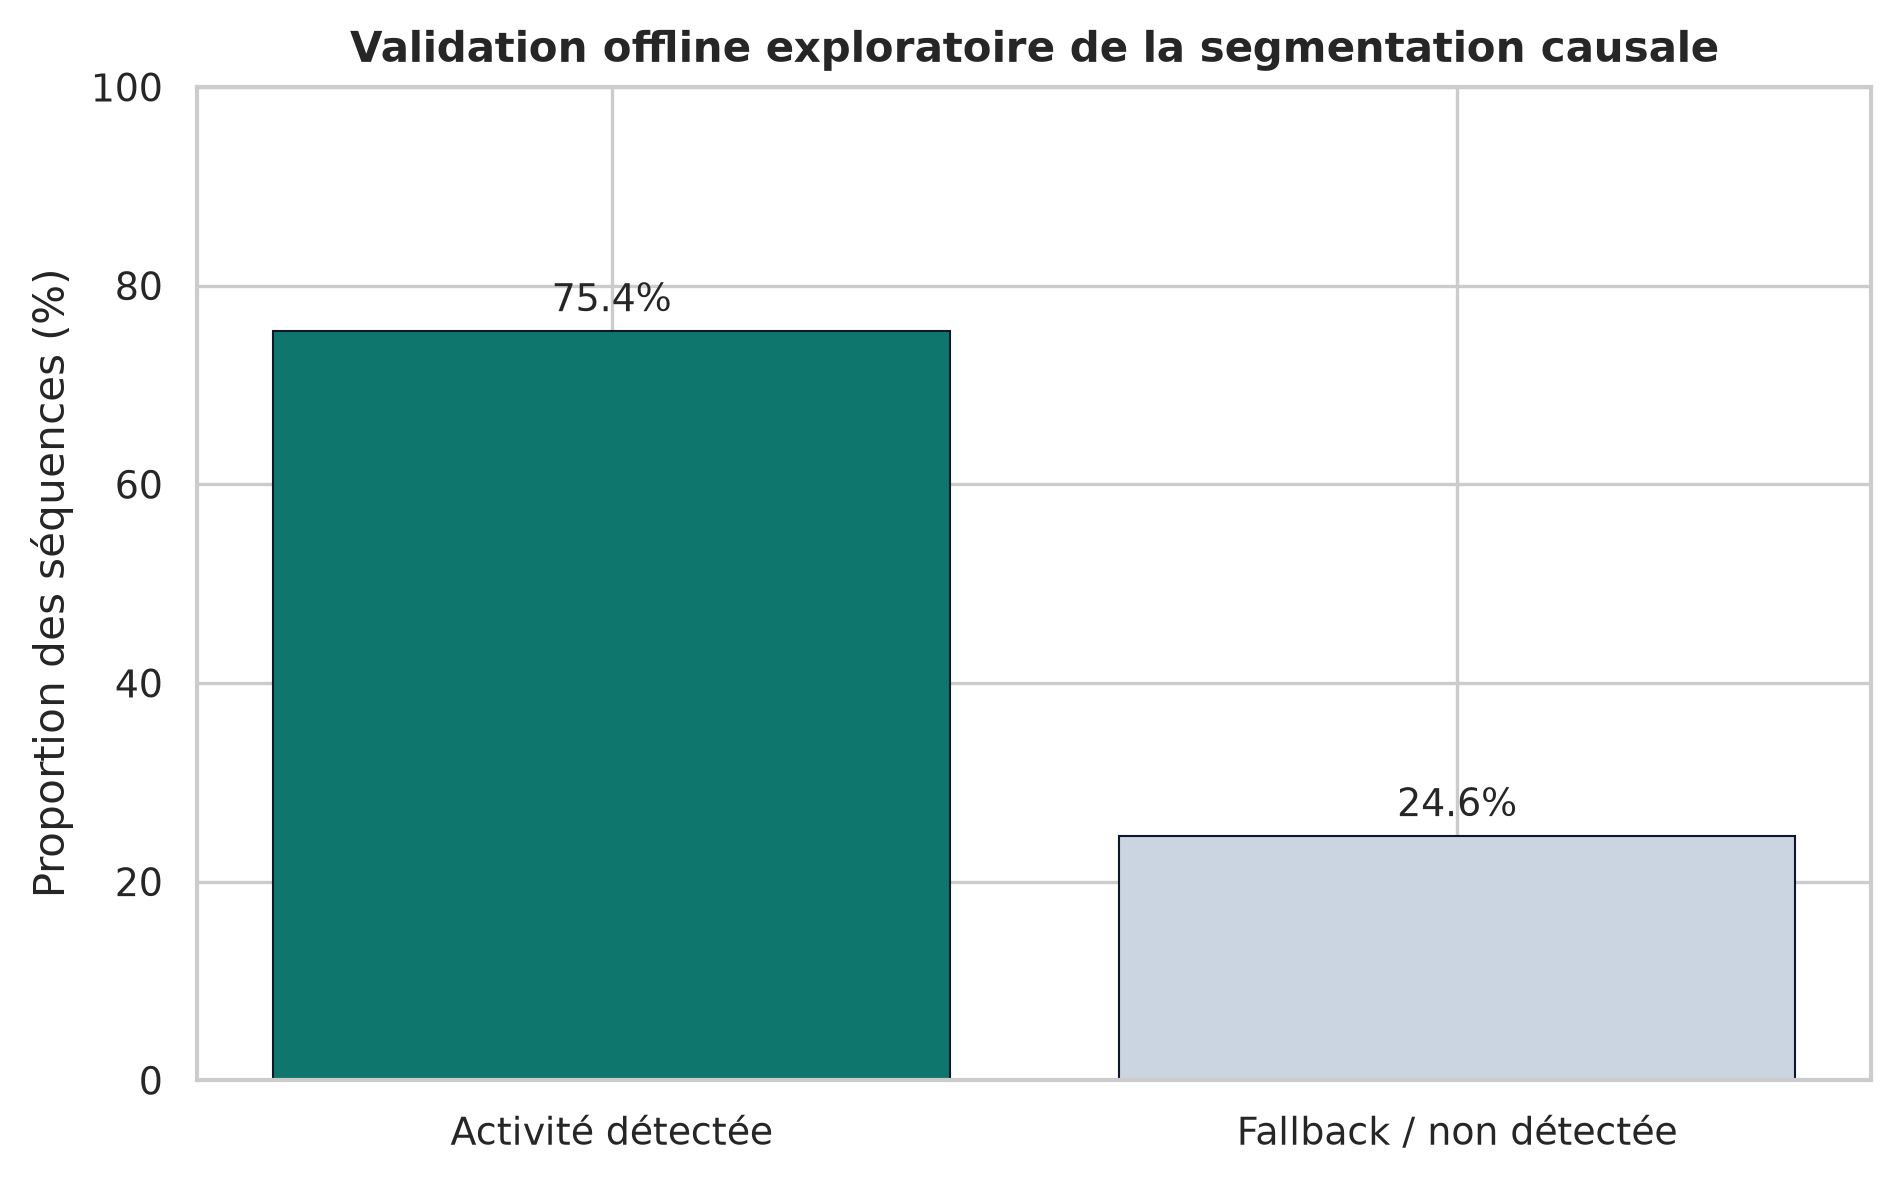
\includegraphics[width=0.94\textwidth]{figures/generated/causal_detection_offline.png}
\caption{Taux de détection de l'activité dans la validation offline exploratoire de la segmentation causale.}
\label{fig:causal-detection}
\end{figure}

La segmentation causale est une condition nécessaire pour une extension continue, mais elle ne suffit pas à transformer la reconnaissance de gloses en traduction. Une véritable traduction continue demanderait des annotations temporelles et linguistiques, une modélisation des transitions et une évaluation spécifique des phrases.

\subsection{Test de robustesse sur le split vidéo officiel}

Un test complémentaire a envoyé à l'API les 5\,957 séquences du split de test officiel. Les séquences proviennent du corpus vidéo LSFB-ISOL après extraction des landmarks autorisés ; elles ne sont donc pas des entrées synthétiques et conservent la diversité des signeurs et des gestes du test verrouillé. Chaque séquence a été rééchantillonnée sur 32 frames, transmise à \texttt{/predict-gru}, puis comparée à son étiquette de référence.

Le test API reproduit exactement les métriques de l'évaluation hors ligne. L'accuracy atteint 82,31\,\%, le macro-F1 0,8153 et la balanced accuracy 0,8129. L'écart nul avec l'audit configuration GRU retenue montre que le chargement des checkpoints, le classement top-3 et le prétraitement déployé ne dégradent pas la performance de classification.

\begin{table}[ht]
\centering
\small
\caption{Résultats détaillés de l'ensemble GRU retenu sur le test API de 5\,957 séquences.}
\label{tab:gru-api-per-class}
\begin{tabular}{lrrrr}
\hline
Glose & Précision & Rappel & F1 & Support \\
\hline
OUI & 0,8420 & 0,8993 & 0,8697 & 1\,013 \\
SOURD & 0,8047 & 0,8925 & 0,8463 & 577 \\
AVOIR & 0,8490 & 0,8224 & 0,8355 & 704 \\
QUOI & 0,8467 & 0,8571 & 0,8519 & 567 \\
REGARDER & 0,7422 & 0,8344 & 0,7856 & 483 \\
NON & 0,8097 & 0,6861 & 0,7428 & 583 \\
DIFFERENT & 0,9085 & 0,9255 & 0,9169 & 322 \\
DIRE & 0,8600 & 0,7559 & 0,8046 & 512 \\
FINIR & 0,7796 & 0,6749 & 0,7235 & 283 \\
BIEN & 0,7787 & 0,8287 & 0,8030 & 327 \\
VOIR & 0,7704 & 0,7822 & 0,7763 & 326 \\
COMPRENDRE & 0,8625 & 0,7962 & 0,8280 & 260 \\
\hline
\end{tabular}
\end{table}

Les résultats par classe montrent que DIFFERENT obtient le meilleur F1 avec 0,9169, suivi d'OUI avec 0,8697 et de QUOI avec 0,8519. Les classes les plus fragiles sont FINIR avec 0,7235 et NON avec 0,7428. La faiblesse de NON provient principalement d'un rappel de 0,6861, ce qui confirme que la confusion NON--SOURD reste une priorité d'amélioration malgré le gain global de la configuration GRU retenue.

La latence HTTP moyenne est de 63,59 millisecondes par séquence, avec une médiane de 59,57 millisecondes. Le P95 est de 86,79 millisecondes et le P99 de 109,41 millisecondes. Le maximum isolé de 758,57 millisecondes constitue une valeur atypique ; il ne doit pas être utilisé comme latence représentative sans une mesure séparée de la charge système. Ces résultats décrivent l'API et l'inférence GRU, mais n'incluent pas l'extraction MediaPipe dans le navigateur ni la synthèse vocale.

Enfin, trois payloads invalides ont été soumis pour vérifier le comportement défensif de l'API : deux formes de matrice incorrectes et un champ \texttt{landmarks} nul. Les trois requêtes ont été rejetées avec le code HTTP 422. Le test confirme donc à la fois la stabilité du modèle sur le split officiel et le respect du contrat d'entrée en cas d'erreur.

\section{Confiance, calibration et rejet}


Le modèle actif n'est pas un seul réseau. Il s'agit d'un ensemble de quinze GRU, obtenu avec trois graines et cinq folds. Pour une séquence, chaque réseau produit un vecteur de douze valeurs réelles avant normalisation. Ces valeurs sont appelées \emph{logits}. Un logit n'est pas une probabilité : il peut être positif ou négatif et mesure seulement la préférence relative du réseau pour une classe.

Chaque vecteur de logits $z^{(m)}$ est converti en distribution par la fonction softmax :
\[
p^{(m)}_c=\frac{\exp(z^{(m)}_c)}{\sum_{j=1}^{C}\exp(z^{(m)}_j)},
\qquad C=12.
\]
Les valeurs $p^{(m)}_c$ sont positives et leur somme vaut un. L'application calcule ensuite la moyenne des quinze distributions :
\[
\bar p_c=\frac{1}{15}\sum_{m=1}^{15}p^{(m)}_c.
\]
La classe affichée est $\hat y=\arg\max_c\bar p_c$. Dans la version actuelle non calibrée, le champ \texttt{confidence} est exactement $\max_c\bar p_c$. Par exemple, si la moyenne donne 0,77 pour OUI, 0,09 pour NON et 0,05 pour COMPRENDRE, l'application affiche OUI avec un score de 0,77. Ce score décrit la préférence probabiliste interne de l'ensemble ; il ne signifie pas encore que 77\,\% des séquences affichées avec ce score sont correctes.

Cette distinction est importante. Les quinze réseaux sont plusieurs entraînements du même type de GRU, et non quinze architectures différentes. Leur diversité vient des graines et des partitions de validation. L'accord de l'ensemble est mesuré séparément par la proportion de réseaux dont la classe top-1 est la classe finale :
\[
\mathrm{Accord}=\frac{1}{15}\sum_{m=1}^{15}\mathbf{1}\!\left(\arg\max_c p^{(m)}_c=\hat y\right).
\]
La marge entre les deux meilleures classes complète ce diagnostic :
\[
\mathrm{Marge}=\bar p_{(1)}-\bar p_{(2)}.
\]

La calibration vise à rapprocher le score affiché de la fréquence réelle de correction. La méthode retenue pour le prototype est la \emph{temperature scaling}. Elle introduit une température positive $T$ avant softmax :
\[
p_{T,c}=\frac{\exp(z_c/T)}{\sum_{j=1}^{C}\exp(z_j/T)}.
\]
Lorsque $T>1$, la distribution est aplatie et les scores trop confiants diminuent. Lorsque $T<1$, elle devient plus concentrée. La valeur $T$ doit être apprise en minimisant la log-vraisemblance négative sur des prédictions hors-échantillon de validation groupée par signeur. Le test officiel ne doit jamais servir à apprendre $T$ ou les seuils de rejet.

Dans l'implémentation actuelle, les sorties probabilistes des quinze réseaux sont d'abord moyennées, puis la température est appliquée à cette distribution agrégée. Le champ \texttt{raw\_confidence} conserve le maximum avant calibration et le champ \texttt{confidence} contient le maximum après calibration lorsqu'un artefact de calibration est présent. Tant que les probabilités hors-échantillon nécessaires ne sont pas archivées, l'API conserve \texttt{confidence\_calibrated=false} et \texttt{accepted=null} ; elle n'invente donc ni température ni seuil à partir du test officiel.

Le rejet est une décision séparée du classement. Il ne change pas la classe top-1 ; il décide seulement si cette classe peut être présentée comme suffisamment fiable. La règle future combinera la confiance calibrée, la marge et l'accord des quinze réseaux :
\[
\mathrm{accept}=\left(\mathrm{confidence}\geq\tau_c\right)\land\left(\mathrm{marge}\geq\tau_m\right)\land\left(\mathrm{accord}\geq\tau_a\right).
\]
Les seuils seront choisis sur validation selon un objectif de couverture fixé à l'avance, par exemple au moins 85\,\% des séquences. Le critère rapporté sera le couple couverture--risque : la couverture est la proportion de séquences acceptées et le risque est le taux d'erreur parmi ces séquences. Un seuil ne sera pas retenu parce qu'il paraît intuitif ; il devra être inscrit avant l'évaluation finale et accompagné d'un intervalle d'incertitude obtenu par bootstrap groupé par signeur.

Pour l'utilisateur, trois états sont préférables à un rejet systématique. Une décision calibrée et séparée est affichée directement. Une décision intermédiaire conserve le top-1 et le top-3, mais désactive la vocalisation automatique. Une décision rejetée demande une nouvelle capture et indique que la capture est incertaine. Cette politique réduit le risque d'afficher une classe fausse comme certaine sans supprimer inutilement les réponses utiles.


\section{Conclusion du chapitre}
L'évaluation récente montre que l'ensemble GRU retenu constitue le meilleur résultat observé, avec un macro-F1 de 0,8153, tandis que le Random Forest complet atteint 0,7839. Le test de robustesse sur les 5\,957 séquences via l'API reproduit exactement ces métriques. La GRU est donc le modèle actif de l'application, tandis que le RF reste conservé comme référence de comparaison et solution de retour arrière.

La calibration isotonic améliore fortement la fiabilité des scores RF, mais ne doit pas être confondue avec une amélioration de la classification. Les anciennes baselines sont utiles pour documenter la progression, mais les conclusions principales du mémoire reposent désormais sur GRU initiale, configuration GRU retenue, Random Forest complet et le test de robustesse API. La prochaine étape est une comparaison à représentation identique, suivie d'une mesure complète de la chaîne webcam et d'une politique de rejet calibrée.

Cette conclusion est une conclusion de reconnaissance contrôlée, pas une preuve de traduction ouverte ni de temps réel strict. Le test API porte sur des landmarks extraits de séquences vidéo et ne mesure pas encore le coût MediaPipe ni la synthèse vocale. La prochaine étape scientifique est donc la validation de la chaîne complète sur des flux webcam réels.

\chapter{Limites et perspectives}

\section{Limites du modèle}

Le GRU de référence de la campagne expérimentale atteint 92,0 \% d'exactitude et un F1-score macro de 0,9181 sur les séquences du signeur réservé au test. Cette mesure concerne un seul découpage et ne garantit pas les mêmes performances pour d'autres signeurs. Le TFLite actuellement déployé dans l'application obtient séparément 90/100 sur les séquences prétraitées du jeu de test ; la correspondance entre ses poids et ceux du nouveau GRU de référence n'est pas établie. Avec quatre personnes dans le corpus, la variabilité des façons de produire les signes reste peu représentée.

Les résultats par classe montrent aussi que la performance varie selon le signe. Tsia et Maty font partie des signes les plus difficiles à reconnaître dans l'évaluation présentée au chapitre 3. Ces erreurs peuvent être liées aux différences de réalisation entre signeurs, mais le corpus ne permet pas d'établir une cause unique. Les points du corps et des mains employés par le modèle ne représentent pas toute l'information linguistique disponible, notamment les expressions du visage et les mouvements de la tête.

Le système traite des signes isolés associés à un vocabulaire fermé de dix classes. Il ne segmente pas une conversation en signes et ne traduit pas des phrases continues. Il ne prend donc pas en compte le contexte linguistique, l'ordre des signes ni les constructions propres à la LSM.

\section{Limites de l'application}

L'application est un prototype de démonstration et non un service déployé en production. La première utilisation de la synthèse vocale nécessite une connexion internet pour charger le modèle ONNX dans le navigateur. Les essais de reconnaissance dépendent également de la qualité de la vidéo et de la détection des landmarks par MediaPipe. Le cadrage, l'éclairage ou une main hors du champ peuvent réduire la quantité d'information disponible pour la prédiction.

La validation de l'application a porté sur un nombre limité de scénarios. Dans les dix essais de l'endpoint décrits au chapitre 4, l'audio est généré pour le résultat disponible, mais la vidéo du signe Miarahaba est classée Solosaina. Ce résultat rappelle que le fonctionnement de la chaîne logicielle ne garantit pas l'exactitude de chaque prédiction. Une campagne de tests plus vaste est nécessaire pour mesurer séparément les erreurs de capture, de détection, de classification et de synthèse.

\section{Limites méthodologiques}

Le corpus comprend 400 séquences pour dix signes et quatre signeurs. Il permet de réserver un signeur au test, mais sa taille ne couvre qu'une partie des variations possibles entre locuteurs. Les captures ont été effectuées dans deux pièces sous un éclairage naturel resté constant, mais le script ne contrôle pas ces conditions et ne documente pas systématiquement le fond ni la distance à la caméra. Les résultats ne permettent donc pas de conclure à la robustesse dans des lieux, éclairages et cadrages variés.

L'évaluation finale porte sur un seul signeur tenu à l'écart de l'entraînement et de la validation. Elle constitue un test de généralisation inter-signeurs, mais ne permet pas d'estimer la performance moyenne sur l'ensemble des personnes utilisant la LSM. Les résultats doivent être interprétés dans ce périmètre.

La campagne expérimentale repose sur un découpage fixe et sur un seul signeur réservé au test. Les écarts entre les trois meilleures exactitudes observées (94,0 \%, 93,0 \% et 92,0 \%) représentent au plus deux séquences sur les 100 du jeu de test. Aucun test statistique ni intervalle de confiance n'a été calculé ; ces résultats ne permettent donc pas d'établir une différence statistiquement significative ni une performance moyenne sur d'autres signeurs. Les comparaisons de taille de modèle sont également limitées par les taux de dropout différents entre configurations. Enfin, la variante à 45 frames est construite par rééchantillonnage des séquences déjà ramenées à 30 frames et n'ajoute pas d'information provenant des vidéos originales.

L'expérience d'augmentation combine du bruit gaussien et un décalage temporel circulaire. L'exactitude du GRU passe de 92,0 \% à 77,0 \%, tandis que celle du LSTM reste à 82,0 \%. Le F1-score macro du LSTM augmenté n'est pas disponible. L'effet propre de chaque transformation ne peut être isolé, et ce résultat ne permet pas de conclure à l'inefficacité de toute augmentation. L'analyse des séquences d'entraînement révèle une discontinuité potentielle aux extrémités dans 206 séquences sur 210 ; elle fournit une piste d'explication pour le jitter, sans établir de lien causal avec la baisse mesurée. Enfin, le TFLite actuellement déployé atteint 90/100 sur les caractéristiques de test, alors que le journal Colab du nouveau GRU de référence annonce 92/100. La correspondance entre les poids de ces deux artefacts n'est pas établie.

\section{Perspectives}

Une première perspective consiste à enrichir le corpus et à évaluer les modèles sur plusieurs signeurs tenus à l'écart, par exemple au moyen d'une validation où le signeur de test varie. Cette évaluation permettrait de mesurer la variabilité des résultats et de vérifier si les scores du modèle mains seules se maintiennent au-delà du découpage actuel. Les différences entre modèles pourraient alors être accompagnées d'intervalles d'incertitude et de comparaisons statistiques adaptées aux prédictions appariées.

Une deuxième perspective est d'étudier les variantes mains seules et à 15 frames comme pistes d'optimisation. Le modèle mains seules a le plus petit nombre de paramètres parmi les trois meilleures configurations, mais son avantage observé doit être confirmé sur un corpus plus large. La fenêtre de 15 frames pourrait réduire le nombre d'étapes récurrentes ; un benchmark sur la machine de démonstration reste nécessaire pour mesurer son effet réel sur la latence et la mémoire. Ces mesures permettraient également de comparer la taille et les performances des modèles après conversion en TFLite.

La reproductibilité du déploiement constitue une autre étape nécessaire. Il conviendrait d'archiver le checkpoint Colab correspondant au GRU de référence à 92,0 \%, de le convertir en TFLite, puis de vérifier que l'artefact obtenu correspond bien au modèle évalué. Le TFLite actuellement présent dans le dépôt obtient 90/100 sur les caractéristiques de test ; tant que la provenance des poids n'est pas reliée au nouveau checkpoint, ces deux scores doivent rester distincts.

Pour l'augmentation des données, des expériences d'ablation pourraient isoler le bruit gaussien du décalage temporel. Des transformations temporelles qui préservent l'ordre et la continuité du geste, ou des perturbations fondées sur la cinématique, pourraient ensuite être étudiées et évaluées sur des signeurs non utilisés pour le réglage. Les résultats actuels ne permettent pas de conclure à l'efficacité de ces méthodes.

À plus long terme, le système pourrait être étendu à la reconnaissance de signes continus. Cette évolution nécessiterait des séquences annotées avec des frontières temporelles et des traductions de référence. Des méthodes telles que la classification temporelle connexionniste (CTC) ou des architectures temporelles pourraient être comparées dans un protocole adapté. Une évaluation avec des utilisateurs de la communauté sourde malgache aiderait également à examiner la pertinence du vocabulaire, des traductions et de la sortie vocale.

\endinput

\begin{conclusion}

Ce mémoire étudie la reconnaissance de signes isolés de la Langue des Signes Malgache à partir de séquences vidéo. Il cherche à déterminer si des points de squelette extraits par MediaPipe permettent de comparer des modèles LSTM et GRU, puis d'intégrer le modèle retenu dans une application restituant le résultat sous forme de texte et de parole malgache.

Dans le cadre expérimental défini, le GRU atteint 90,0 \% d'exactitude et un F1-score macro de 0,897 sur les 100 séquences de test produites par un signeur absent de l'entraînement. Le LSTM atteint respectivement 87,0 \% et 0,864. Le GRU compte 137\,610 paramètres, contre 182\,538 pour le LSTM. Ces résultats motivent le choix du GRU pour le prototype. Ils concernent dix signes isolés et un seul signeur de test ; ils ne démontrent pas une reconnaissance générale de la LSM ni une traduction de phrases continues.

Le travail apporte un corpus de 400 séquences réparties entre quatre signeurs, un pipeline de préparation des données et une comparaison expérimentale de deux modèles récurrents. Il comprend également une application web composée d'un backend FastAPI utilisant le modèle converti au format TFLite et d'un frontend qui produit la synthèse vocale malgache dans le navigateur.

La validation de l'application confirme le fonctionnement des composants sur le scénario essayé, tout en mettant en évidence une erreur de classification sur la séquence de référence. L'effectif du corpus, le nombre de signeurs et la diversité limitée des conditions de capture restreignent la portée des conclusions. Le prototype doit donc être considéré comme une démonstration de faisabilité pour un vocabulaire fermé.

Les suites prioritaires sont d'élargir le corpus, d'évaluer le modèle sur plusieurs signeurs jamais vus et de tester l'application dans des conditions de capture variées. À plus long terme, des séquences annotées de signes continus permettraient d'étudier une traduction en contexte. La collaboration avec les signeurs malgaches sera nécessaire pour valider le vocabulaire et les résultats d'usage.

\end{conclusion}

\appendix
\setcounter{chapter}{0}
\chapter{Extraits du code du prototype LSM}

Cette annexe rassemble des extraits représentatifs du code réellement utilisé
dans le prototype LSM.

\section{Extraction des points de pose et des mains}

Le traitement vidéo conserve les dernières coordonnées disponibles lorsqu'un
repère n'est temporairement pas détecté. Les 33 points du corps et les 21 points
de chaque main forment 225 valeurs par image.

\begin{verbatim}
if results.pose_landmarks:
    corps = np.array([
        [lm.x, lm.y, lm.z]
        for lm in results.pose_landmarks.landmark
    ])
    derniere_pose = corps
else:
    corps = derniere_pose
    n_sans_detection += 1

vecteur = np.concatenate([
    corps.flatten(),
    main_g.flatten(),
    main_d.flatten()
])
frames.append(vecteur)
\end{verbatim}

\section{Rééchantillonnage et normalisation}

Les séquences sont ramenées à 30 frames. À chaque frame, les coordonnées sont
centrées sur le milieu des épaules et divisées par la distance entre celles-ci.

\begin{verbatim}
indices = np.linspace(0, len(sequence) - 1, n_cible)
sequence = np.array([
    sequence[int(round(index))] for index in indices
])

for frame_index in range(sequence.shape[0]):
    epaule_g = sequence[frame_index, 33:36]
    epaule_d = sequence[frame_index, 36:39]
    centre = (epaule_g + epaule_d) / 2.0
    distance = np.linalg.norm(epaule_g - epaule_d)
    if distance < 1e-6:
        distance = 1.0
    for point_index in range(0, 225, 3):
        sequence[frame_index, point_index:point_index + 3] = (
            sequence[frame_index, point_index:point_index + 3] - centre
        ) / distance
\end{verbatim}

\section{Conversion du modèle Keras en TFLite}

Le script de conversion conserve les poids appris, active l'optimisation
TFLite et vérifie l'artefact avec un interpréteur avant son écriture.

\begin{verbatim}
model = tf.keras.models.load_model(args.model, compile=False)
model = make_tflite_compatible_model(model, tf)
converter = tf.lite.TFLiteConverter.from_keras_model(model)
converter.optimizations = [tf.lite.Optimize.DEFAULT]
model_content = converter.convert()

interpreter = tf.lite.Interpreter(model_content=model_content)
interpreter.allocate_tensors()
args.output.parent.mkdir(parents=True, exist_ok=True)
args.output.write_bytes(model_content)
\end{verbatim}

\section{Inférence TFLite}

L'interpréteur est initialisé une fois au démarrage du backend. Son accès est
sérialisé pendant l'inférence et la classe présentant la probabilité maximale
est renvoyée avec son score.

\begin{verbatim}
with _INTERPRETER_LOCK:
    INTERPRETER.set_tensor(INPUT_DETAILS["index"], batch)
    INTERPRETER.invoke()
    probabilites = INTERPRETER.get_tensor(
        OUTPUT_DETAILS["index"]
    )[0]

index = int(np.argmax(probabilites))
return {
    "signe": CLASSES[index],
    "confiance": float(probabilites[index]),
}
\end{verbatim}

\section{Endpoint FastAPI}

L'endpoint reçoit le clip vidéo sous forme de fichier multipart et délègue le
traitement au module d'inférence. Les vidéos non exploitables sont renvoyées
comme erreurs de requête.

\begin{verbatim}
@app.post("/predire")
def predire_endpoint(file: UploadFile = File(...)):
    video_bytes = file.file.read()
    try:
        return predire(video_bytes)
    except InvalidVideoError as error:
        raise HTTPException(
            status_code=422, detail=str(error)
        ) from error
\end{verbatim}

\section{Capture webcam et appel de l'API}

Le navigateur enregistre un clip à partir du flux webcam puis l'envoie à
l'endpoint de prédiction avec \texttt{FormData}.

\begin{verbatim}
const chunks = [];
recorder.addEventListener("dataavailable", (event) => {
  if (event.data.size > 0) chunks.push(event.data);
});
recorder.start();
window.setTimeout(() => {
  if (recorder.state === "recording") recorder.stop();
}, captureDurationMs());

const formData = new FormData();
formData.append("file", clip, "capture.webm");
const response = await fetch("/predire", {
  method: "POST",
  body: formData,
});
\end{verbatim}

\section{Synthèse vocale et création du fichier WAV}

Le texte prédit est vocalisé dans le navigateur avec Transformers.js et le
modèle ONNX malgache. Le signal produit est converti en WAV PCM pour le lecteur
audio HTML.

\begin{verbatim}
const { pipeline, env } = await import(
  "https://cdn.jsdelivr.net/npm/@xenova/transformers"
);
env.backends.onnx.wasm.numThreads = 1;
const synthesizer = await pipeline(
  "text-to-speech",
  "elloza/mms-tts-mlg-onnx",
  { quantized: true }
);
const speech = await synthesizer(text);
audioResult.src = URL.createObjectURL(
  makeWav(speech.audio, speech.sampling_rate)
);
\end{verbatim}

\endinput

\chapter{Corpus LSFB-ISOL}

\section{Catalogue général du corpus}
\begin{verbatim}
{
  "source": "LSFB-ISOL",
  "instance_count": 13547,
  "signer_count": 99,
  "fields": ["id", "sign", "signer", "start", "end"],
  "partitions": {
    "train": 7590,
    "test": 5957,
    "shared_signers": 0
  }
}
\end{verbatim}

\section{Extrait brut d’instances LSFB-ISOL}
\begin{verbatim}
id,sign,signer,start,end
CLSFBI0104A_S001_B_253439_253802,OUI,S001,253439,253802
CLSFBI0103A_S002_B_165985_166679,NON,S002,165985,166679
CLSFBI0103A_S001_B_367470_367816,SOURD,S001,367470,367816
CLSFBI0104A_S001_B_479609_479848,QUOI,S001,479609,479848
CLSFBI0104A_S002_B_476347_476533,AVOIR,S002,476347,476533
CLSFBI0103A_S001_B_335087_335232,DIRE,S001,335087,335232
CLSFBI0103A_S001_B_295863_296869,REGARDER,S001,295863,296869
CLSFBI0103A_S002_B_189863_190520,COMPRENDRE,S002,189863,190520
CLSFBI0103A_S001_B_466550_466747,FINIR,S001,466550,466747
CLSFBI0111A_S001_B_220590_220803,BIEN,S001,220590,220803
CLSFBI0103A_S002_B_139019_139281,VOIR,S002,139019,139281
CLSFBI0103A_S001_B_286621_286862,DIFFERENT,S001,286621,286862
\end{verbatim}

\section{Structure d’une séquence de landmarks}
\begin{verbatim}
{
  "landmark_order": [
    "pose_0..pose_32",
    "left_hand_0..left_hand_20",
    "right_hand_0..right_hand_20"
  ],
  "coordinates": 3,
  "frames": 32,
  "values_per_frame": 225,
  "classes": 12
}
\end{verbatim}

\section{Séparation des signeurs}
\begin{verbatim}
{
  "train_signers": 59,
  "test_signers": 40,
  "shared_signers": 0,
  "duplicate_instance_ids": 0,
  "duplicate_row_hash_count": 0
}
\end{verbatim}


\newpage
\begin{spacing}{1}
  \bibliographystyle{plain}
  \addcontentsline{toc}{chapter}{BIBLIOGRAPHIE}
  \bibliography{biblio/bibliographie}
\end{spacing}
\newpage
\begin{spacing}{1}
  \nociterefs{*}
  \bibliographystylerefs{alphaurl}
  \addcontentsline{toc}{chapter}{WEBOGRAPHIE}
  \bibliographyrefs{biblio/webographie}
\end{spacing}
\end{document}
